\documentclass{report}
\usepackage[utf8]{inputenc}
\usepackage{amsmath}
\usepackage{graphicx}
\usepackage{pdfpages}
\usepackage{listings}
\usepackage{fancyhdr}
\usepackage{titling}
\usepackage[margin=1.0in]{geometry}

\DeclareMathOperator\erf{erf}
\DeclareMathOperator\erfc{erfc}

\pagestyle{fancy}
\fancyhf{}
\rhead{\theauthor}
\rfoot{Page \thepage}
\lhead{\thetitle, Lecture \thechapter}

\title{MATH 316 Notes}
\author{Ashtan Mistal}
\date{May - June 2021}

\begin{document}

\maketitle

\tableofcontents{}

\chapter{Lecture 1}
\graphicspath{{./Lecture1/}}
Some basic, quick notes regarding the course:

\begin{itemize}
    \item Watch the pre-recorded lectures prior to the actual lectures
    \item Homeworks: 20\%; Midterm: 30\%; Final: 50\%
    \item Homeworks are best 4 out of 5
    \item Exams will be open book, open notes
    \item Homeworks can be written + scanned, or written using OneNote or \LaTeX
\end{itemize}

\section{Brief Overview of ODEs}

First Order ODEs

\begin{itemize}
    \item Separable ODEs (ex: $y' = \frac{dy}{dx} = p(x) \cdot q(y)$
    \item Linear: $Ly = y' + p(x) y = Q(x)$, where $\underbrace{L}_{\text{linear}} = \frac{d}{dx} + p(x)$
\end{itemize}

Second Order ODEs:

\begin{itemize}
    \item Constant coefficient ODE: $Ly = y'' + a y' + by = 0$
    \item Cauchy-Euler, or Equi-dimensional ODEs: $Ly = x^2 y'' + a x y' + by = 0$
    \item L is the linear operator. In the constant coefficient, $L = \frac{d^2}{dx^2} + a \frac{d}{dx} + b$ 
\end{itemize}

\subsection{Examples}
\subsubsection{First Order Separable Equation Examples}

$\frac{dy}{dx} = p(x) Q(y) \longrightarrow \int{\frac{dy}{Q(y)}} = \int{P(x) dx + C}$

Then, we get:

$\frac{dy}{dx} = y \cos(x) \rightarrow \frac{dy}{y} = \cos(x) dx \longrightarrow \ln{|y|} = \sin(x) + C \rightarrow y = C_1 e^{\sin(x)}$

\subsubsection{Linear First Order Equation:}

$y' + p(x) y = Q(x)$

Multiply both sides by an integrating factor $\mu(x)$

Ex: $y' + \frac{2x}{1 + x^2} y = \frac{\cot(x)}{1 + x^2}$
$\mu(x) y' + \underbrace{\mu(x) \frac{2x}{1 + x^2} y}_{\mu'(x) y} = \frac{\cot(x)}{1 + x^2} \mu(x)$
Compare to: $\mu(x) y' + \mu'(x) y = \left[\mu(x) y(x) \right]'$

$\frac{d \mu}{dx} = \mu \frac{2x}{1 + x^2}$: integrate: $\int{\frac{d \mu}{\mu}} = \int{\frac{2x}{1 + x^2} dx + C}$

Hence, using integrating factor: $$ \ln |\mu(x)| = \ln(1 + x^2) + C$$ with $\mu(x) = C_1 (1 + x^2)$

Hence, $$C_1(1 + x^2) y' + C_1 2xy = C_1 \cot(x)$$

$$\frac{d}{dx} \left[ (1 + x^2) y \right] = \cot(x)$$

$$(1+x^2)y = \int \cot(x) + C = \ln|\sin(x)| + C$$

Hence, $$y(x) = \frac{\ln|\sin(x)|}{1+x^2} + \frac{C}{1+x^2}$$

\subsection{Second Order Constant Coefficient ODE}

$$ay'' + by' + cy = 0$$

We start with a guess: $e^{rx}$, and substitute: $(ar^2 + br + c) \cdot e^{rx} = 0$. Note that $ar^2 + br + c$ is the characteristic equation. We then have two solutions:'

$$r_{1,2} = \frac{-b \pm \sqrt{b^2 - 4ac}}{2a}, \Delta = b^2 - 4ac$$

Based on the sign of $Delta$, we have 3 different cases:

\begin{itemize}
    \item $\Delta > 0$: 2 real, distinct roots
    \item $\Delta < 0$: 2 complex roots
    \item $\Delta = 0$: Repeated roots. 
\end{itemize}

Example: $2y'' + 2y' + y = 0$: Guess $e^{rx}$. 

$2r^2 + 2r + 1 = 0 \longrightarrow r_{1,2} = \frac{-2 \pm \sqrt{4 - 8}}{2(2)}, \Delta = -4$. As $-4 < 0$, this is 2 complex roots. We end up with the following solution: $$e^{\frac{-x}{2}} \left[C_1 e^{\frac{i}{2} x} + C_2 e^{\frac{-i}{2} x} \right]$$

Using Euler's formula $e^{i \theta} = \cos(\theta) + i \sin(\theta)$, we get the following: $$e^{\frac{-x}{2}} \left[ C_1 (\cos(\frac{x}{2}) + i \sin(\frac{x}{2})) + C_2 (\cos(\frac{x}{2}) - i \sin(\frac{x}{2})) \right]$$

$$e^{\frac{-x}{2}} \left[(C_1 + C_2) \cos(\frac{x}{2}) + i (C_1 + C_2) \sin(\frac{x}{2}) \right]$$

$$y(x) = e^{\frac{-x}{2}} \left[ A_1 \cos{\frac{x}{2}} + A_2 \sin{\frac{x}{2}} \right]$$

Real form of the solution, A1 \& A2: $c_1 = a_1 + i b_1$; $c_2 = a_2 + i b_2$

$A_1 = (a_1 + a_2) + i (b_1 + b_2)$, and $A_2 = i(a_1 - a_2) - (b_1 - b_2)$. $b_1 + b_2 = 0$, $a_1 - a_2 = 0$

\hfill \break
Example: $y'' - 2y' + y = 0$. Characteristic equation: $r^2 - 2r + 1 = 0 \longrightarrow (r - 1)^2 = 0$, and therefore the roots are $r = 1$ repeated. Hence, 

$$y = C_1 e^{x} + C_2 x e^x$$

is the solution of the equation. 

\subsubsection{Cauchy - Euler Eqn}

$$Ly = x^2 y'' + \alpha x y' + \beta y = 0$$

Guess: $y = x^r$

EX: $2x^2 y'' - x y' + y = 0$. $y(x) = x^r, y'(x) = r x^{r-1}, y'' = r(r-1) x^{r-2}$.

Therefore, $$2 r (r-1)x^r - rx^r + x^r = 0$$

which is equivalent to $$\left[2r(r-1) - r + 1 \right] x^2 = 0$$

$$2r(r-1) - r + 1 = 0 \longrightarrow 2r^2 - 3r + 1 = 0$$

$$r_{1,2} = \frac{3 \pm \sqrt{9 - 8}}{2(2)} = 1, \frac{1}{2}$$

Hence, the solution to the equation is $y(x) = C_1 x + C_2 x^{\frac{1}{2}}$

\hfill

EX2: $x^2 y'' - x y' + y = 0$

$y(x) = x^r$ hence, we get: $r(r-1)x^r - rx^r + x^r = 0$.

Therefore $\left[r(r-1) - r + 1 \right]x^r = 0$. 

$$r^2 - 2r + 1 = (r-1)^2 = 0 \rightarrow r = 1$$

$$y_1 = x, y_2 = \ln(x) \cdot x$$

$$y(x) = C_1 x + C_2 x \ln(x)$$

(?) $L y = 0, L \frac{d}{dr} y(x,r) = 0, \frac{d}{dr}(x^r) = x^r \ln(x)$

\hfill 

EX3: $x^2 y'' - x y' + 5y = 0$. 
$y(x) = x^r$, and therefore $r(r-1)x^2 - r x^r + 5 x^r = 0$

$\left[r(r-1) - r + 5 \right] x^r = 0$, hence, $r^2 - 2r + 5 = 0$. We then get the general solution of the following:

$$y(x) = C_1 x^{1 + 2i} + C_2 x^{1 - 2i}$$

This can be re-written as the following:

$$y(x) = x \left[ C_1 e^{2i \ln(x)} + C_2 e^{-2i \ln(x)} \right]$$

And hence as the following:

$$y(x) = x \left[ C_1 (\cos(2 \ln (x) + i \sin(2 \ln(x)) + C_2 (\cos(2 \ln(x)) - i \sin(2 \ln(x))) \right]$$

$$ = x \left[(c_1 + c_2) \cos(2 \ln(x)) + i (c_1 - c_2) \sin(2 \ln(x)) \right]$$

$$ = x \left[A_1 \cos(2 \ln(x)) + A_2 \sin(2 \ln(x)) \right]$$

$A_1$ and $A_2$ are real. 

\hfill

\hfill

EX4: Solve the IVP

$$x^2 y'' - 3 xy' + 4y = 0, y(1) = 1, y'(1) = 1$$

If we let $y(x) = x^r$, then we get the following: $y(x) = x^r, y'(x) = r x^{r-1}, y'' = r(r-1) x^{r-2}$

Plugging this into our equations:

$x^2 r(r-1) x^{r-2} - 3 xr x^{r-1} + 4 x^r = 0$

Solving, we discover we have a repeated root of 2. Hence, the general solution is $y(x) = C_1 x^2 + C_2 x^2 \ln(x)$. Plugging in the initial conditions, we find that $C_1 = 1$, and $C_2 = -1$ and hence the solution is $y(x) = x^2 - x^2 \ln(x)$

\section{Series Solutions of ODEs}

We use power series expansion to solve variable coefficient linear ODEs. Remember that a function $f(x)$ can be approximated by a polynomial of degree $n$, such that $f(x) = a_0 + a_1 x + a_2 x^2 + ... + a_n x^n$. As the degree of $n$ increases, the approximation improves. Hence, $f(x) = \sum_{m = 0}^{\infty} a_m x^m$. Or, in general, we can approximate $f(x)$ by a power series expanded about a point $x_0$, writing it as $f(x) = \sum_{n = 0}^{\infty} a_n (x - x_0)^n$. We can remember that when we had the Taylor series, $a_n = \frac{f^{(n)} (x_0)}{n!}$. So, we have: $f(x) = \sum_{n = 0}^{\infty} \frac{f^{(n)} x(0)}{n!} (x - x_0)^n$.

\subsubsection{Example: $y' + (1 - 2x) y = 0$}

Using the integrating factor, $\mu(x) = e^{\int (1 - 2x) dx} = e^{x - x^2}$. 

$\left[ y e^{x - x^2} \right]' = 0 \longrightarrow y e^{x - x^2} = C \rightarrow y = C e^{-x + x^2}$. 

Use Taylor expansion $y(x)$ about the point $x_0 = 0$. 

In order to do this, we write it as the sum described above:

$$f(x) = \sum_{n = 0}^{\infty} \frac{f^{(n)} x(0)}{n!} (x - x_0)^n$$

We can then let $y = \sum_{n = 0}^{\infty} \frac{f^{(n)} x(0)}{n!} x^n$ and $y' = \sum_{n = 1}^{\infty} \frac{f^{(n)} x(0)}{n!} n x^{n-1}$, and therefore we can write our ODE as $$\sum_{n = 1}^{\infty} \frac{f^{(n)} x(0)}{n!} x^{n-1} + (1 - 2x)\sum_{n = 0}^{\infty} \frac{f^{(n)} x(0)}{n!} x^n = 0$$


\chapter{Lecture 2}
\graphicspath{{./Lecture2/}}
\section{Solving the problem from last class}

We started with a simple example that was solvable using integrating factor, and we are now going to do the Taylor expansion of the \textbf{answer}, around the point $x = x_0$. THe confusion from last class was that we tried to solve the ODE using a Taylor expansion \textbf{of the differential equation}, as opposed to the actual answer. 

$$y(x) = y(0) + \frac{y'(0)}{1} x + \frac{y''(0)}{2!} x^2 + ...$$

$$y(x) = C \left[1 - x + \frac{3}{2} x^2 - \frac{7}{6} x^3 + ... \right]$$

From the class notes:

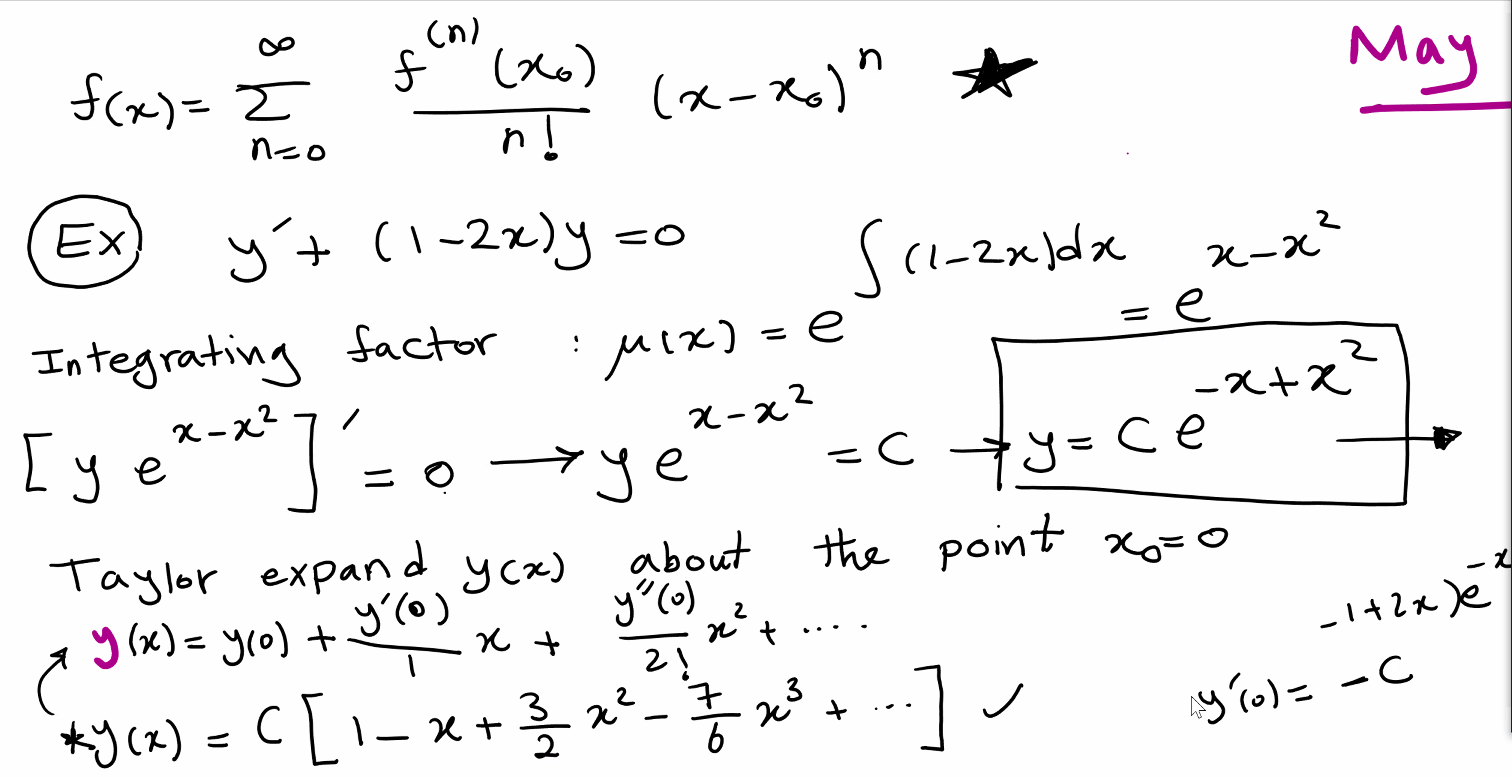
\includegraphics[width = 0.9 \textwidth]{image1.png}

Note that we factored C out of the taylor expansion. Moving forward, assume $y(x) = \sum_{n = 0}^{\infty} a_n x^n$. 

$$y' + (1 - 2x) y = 0$$

$$y' + y - 2xy = 0$$

$$\text{letting } y = \sum_{n = 0}^{\infty} a_n x^n, \text{ and } y' = \sum_{n = 1}^{\infty} a_n n x^{n-1}$$

$$\sum_{n = 1}^{\infty} a_n \underbrace{n}_{m = n-1; n = 1, m = 0} x^{n-1} + \sum_{n = 0}^{\infty} \underbrace{a_n}_{m = n} x^n - 2 \sum_{n = 0}^{\infty} \underbrace{a_n}_{m = n+1;  n = 0, m = 1} x^{n+1} = 0$$

Not exactly sure what these variables are doing with the $n$ and $m$... I guess they're dummy variables that we're using for each sum. 

$$ \sum_{m = 0}^{\infty} a_{m+1} (m+1)x^m + \sum_{m = 0}^{\infty} a_m x^m - 2 \sum_{m = 1}^{\infty} a_{m-1} x^m = 0$$

Peel-off:

$$a_1 x^0 + a_0 x^0 + \sum_{m = 1}^{\infty} \left[a_{m+1} (m+1) + a_m - 2 a_{m-1} \right] x^m = 0$$

Note that $x^0, x, x^2, ..., x^n$ are linearly independent. 

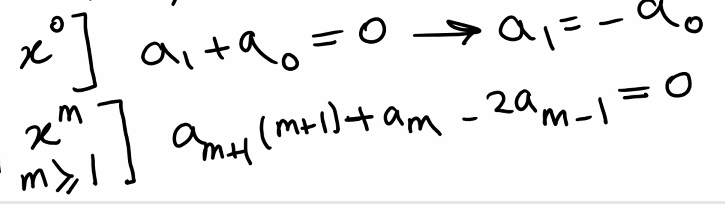
\includegraphics[width = 0.7 \textwidth]{image2.png}

Q: Why do we need to shift the indices?

A: We want to get to a single sigma -- A single sum. If we don't do it, we aren't able to get to a single relation. Indices must start at the same point to be able to combine sums. 

From the relation $a_{m=1} (m+1) + a_m - 2 a_{m-1} = 0$, we can find the relation:

$$a_{m+1} = \frac{-a_m + 2 a_{m-1}}{m+1}$$

$$m = 1: a_2 = \frac{-a_1 + 2 a_0}{2} = \frac{3}{2} a_0$$

$$m = 2: a_3 = \frac{-a_2 + 2 a_1}{3} = \frac{-7}{6} a_0$$

$$y(x) = a_0 + a_1 x + a_2 x^2 + a_3 x^3 + ...$$

$$ y(x) = a_0 - a_0 x + \frac{3}{2} a_0 x^2 - \frac{7}{6} a_0 x^3 + ...$$

$$y(x) = a_0 \left[ 1 - x + \frac{3}{2} x^2 - \frac{7}{6} x^3 + ... 
\right]$$

$$ = \text{Taylor expansion of the direct solution}$$

\section{Example 2}

$$ x y' + (2 - x) y = 0$$

$$ y' + \frac{2-x}{x} y = 0$$

Solving this using integrating factor method, we find the following:

$$\mu(x) = e^{\int \frac{1-x}{x} dx} = e^{2 \ln x - x} = x^2 e^{-x}$$

$$\left[x^2 e^{-x} y \right]' = 0 \rightarrow y = \frac{C}{x^2 e^{-x}} = C x^-2 e^x$$

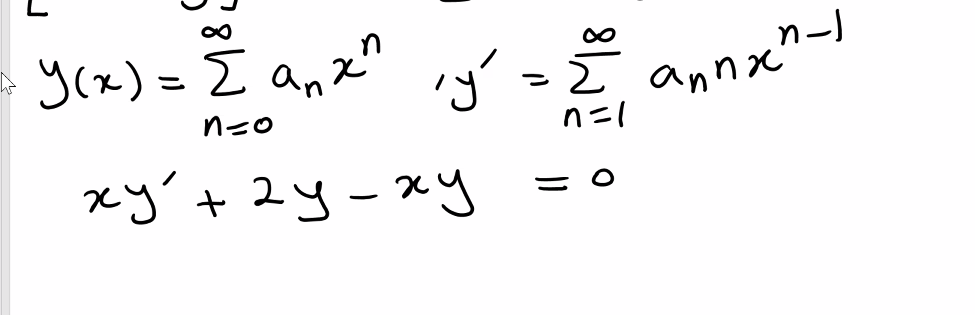
\includegraphics[width = 0.9 \textwidth]{image3.png}

$$\sum_{n = 1}^{\infty} a_n n x^n + 2 \sum_{n = 0}^{\infty} a_n x^n - \sum_{n = 0}^{\infty} a_n x^n+1 = 0$$

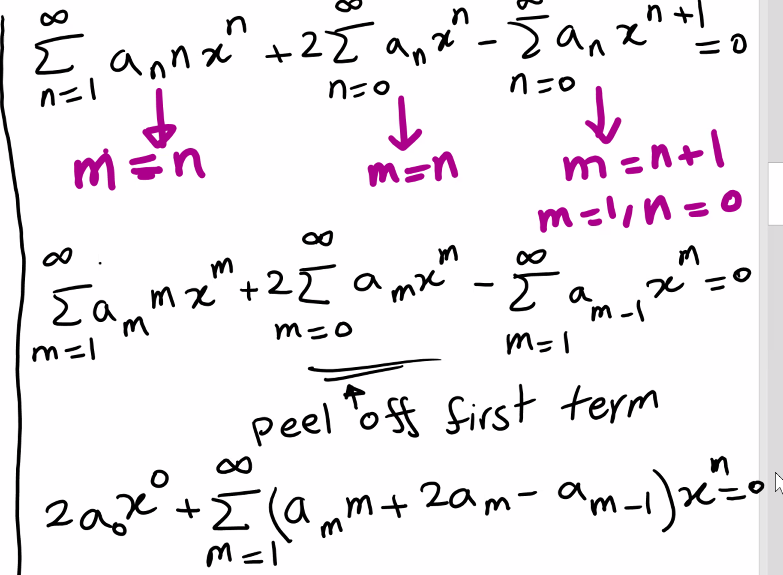
\includegraphics[width = 0.9 \textwidth]{image4.png}

$$\left. x^0 \right] 2 a_0 = 0 \longrightarrow a_0 = 0$$

$$ \left. \begin{matrix} x^m \\ m \geq 1 \end{matrix} \right] a_m (m+2) = a_{m-1}$$

$$\text{note that } a_m = \frac{a_{m-1}}{m+2} \text{for m} \geq 1$$

$$m = 1: a_1 = \frac{a_0}{3} = 0$$

$$m = 2: a_2 = \frac{a_4}{4} = 0$$

This is a trivial solution; they are all zero (and will continue to be). 

$y = c x^{-2} e^x$ is the general solution. 

$$ = C \underbrace{x^{-2}}_{\text{Capture the singularity}} \underbrace{\left[ 1 + x + \frac{x^2}{2!} + \frac{x^3}{3!} + ... \right]}_{\sum_{n = 0}^{\infty} a_n x^n}$$

$$ y(x) = \underbrace{x^r}_{\text{Capture singularity}} \sum_{n = 0}^{\infty} a_n x^n$$

This brings us to the \textbf{Forbenius Series}. 

\section{Forbenius Series}

Let's define ordinary \& singular points:

A linear 2nd order ODE:

$$P(x) y'' + Q(x) y' + r(x) y = 0$$

$$y'' + \frac{Q(x)}{P(x)} y' + \frac{R(x)}{P(x)} y = 0$$

Letting $p(x) = \frac{Q(x)}{P(x)}$ and $q(x) = \frac{R(x)}{P(x)}$. If they are both \textbf{analytic} at the point $x_0$. i.e. they have Taylor expansions about $x_0$, $x_0$ is an ordinary point. Otherwise, $x_0$ is a singular point. 

Example: $\left. \begin{matrix} p(x) = \frac{1}{x} \\ p(x) = \ln(x) \end{matrix} \right\} \text{At } x = 0 \text{, not analytic}$.

Analytic means that is is expressible as a power series around $x_0$. It means that it is infinitely differentiable around $x_0$. 

\subsubsection{Quick notes}

\begin{itemize}
    \item A power series solution is possible for all ordinary points (similar to the first example we saw), but not all singular points. 
    \item For singular points, we introduce the Forbenius Series. However, this only works for some singular points. 
    \item Singular points results in the change of the nature of the ODE. Ordinary points exists in the domain of $p(x)$ and $q(x)$. 
    \item The radius of convergence of the power series is at least as large as the distance from the $x_0$ to the nearest singular point.
    \begin{itemize}
        \item For example, when we had $y = C x^{-2} e^x$, we realize that $x=  0$ is a singular point. 
        \item We can see this in both the answer as well as the ODE. \item When we plot the function, it looks like this:
        \item 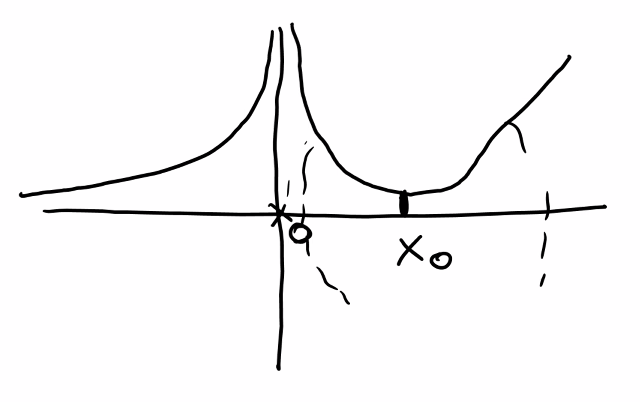
\includegraphics[width = 0.5 \textwidth]{image6.png}
        \item The dotted circles around $x_0$ is the radius of convergence. 
    \end{itemize}
\end{itemize}

Example:

$$y' + (1 - 2x)y =0$$

$$y(x) = C e^{-x + x^2}$$

There are no singular points. Hence the radius of convergence is infinity. 

\subsection{Singular Points}

Singular points are divided into two classes:

\begin{itemize}
    \item Regular singular points, that we use the Forbenius series solution for
    \item Irregular singular points (Beyond this course). For these, we \textbf{cannot} use Forbenius series. 
\end{itemize}

\chapter{Lecture 3}
\graphicspath{{./Lecture3/}}
\section{Singular Points}

Singular points are divided into two classes:

\begin{itemize}
    \item Regular singular points, where we use the Frobenius series solution
    \item Irregular singular points, which are beyond the scope of the course
\end{itemize}

If we are to look at the ODE $P(x) y'' + Q(x) y' + R(x) y = 0$, and define the point $x_0$ as a singular point, we have the following:

The Cauchy-Euler equation is 

\begin{equation}
\label{Cauchy-Euler}
    (x - x_0)^2 + \alpha (x - x_0) y' + \beta y = 0
\end{equation}

We know that $y = (x - x_0)^r$ (As an example). 

How do we make $P(x) y'' + Q(x) y' + R(x) y = 0$ look like( \ref{Cauchy-Euler})?

If we multiply with $(x - x_0)^2$ and divide by $P(x)$, we may get something similar to the Cauchy-Euler. 

Then, we get something like this:
\begin{equation}
    (x - x_0)^2 y'' + \left\{ \frac{Q(x)}{P(x)} (x - x_0) \right\} (x - x_0) y' + \left\{ \frac{R(x)}{P(x)} (x - x_0)^2 \right\} y = 0
\end{equation}


Now, if $\frac{Q(x)}{P(x)}(x - x_0)$ and $\frac{R(x)}{P(x)} (x - x_0)^2$ are analytic at $x = x_0$, then the singularity is not worse than the singularity in the Cauchy-Euler equation (\ref{Cauchy-Euler}), \textbf{and} $x_0$ is a "regular singular point". Otherwise, $x_0$ is an "irregular singular point". 

If we start to write the Taylor series for (?),

$\frac{Q(x)}{P(x)} (x - x_0) = p_0 + p_1 (x - x_0) + ...$

$\frac{R(x)}{P(x)} (x - x_0)^2 = q_0 + q_1 (x - x_0) + ...$

Being analytic means that we need to be able to write the series. 

An example of a singular point:

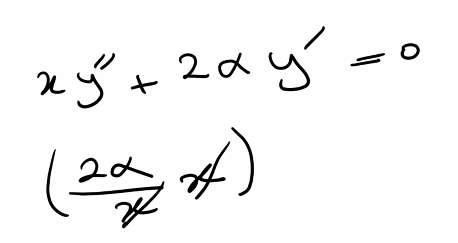
\includegraphics[width = 0.6 \textwidth]{image1.png}

Here, $x = 0$ is a singular point. (We re-wrote the first equation as the second equation, I believe)

\hfill \break

As $x \longrightarrow x_0$, our ODE becomes: $(x - x_0)^2 y'' + p_0 (x - x_0) y' + q_0 y = 0$

The corresponding Cauchy-Euler equation solution: $y = (x - x_0)^r$. We need to have finite $p_0$ and $q_0$. If $p_0$ and $q_0$ are both finite, then $x_0$ is a regular singular point. Otherwise, it is an irregular singular point. 

For regular singular points, the solution we are going to write: 

$$\underbrace{y(x) = (x - x_0)^r}_{*} \underbrace{\sum_{n = 0}^{\infty} a_n (x - x_0)^n}_{\text{Correction}}$$

*: The singular part of the solution to the corresponding Cauchy-Euler. 

\subsection{Example}

$$x(1+x^2) y'' + 2xy' + (1+x^2) y = 0$$. 

Classify singular points. Here, $p(x) = x(1+x)^2$, $Q(x) = 2x$, and $R(x) = 1+x^2$. Singular points: $\left\{ \begin{matrix} x = 0 \\ x = \pm i \end{matrix} \right.$ We need $p(x_0) = 0$ (Take a look at the left hand side if you don't understand!). 

Classify them:

$\left\{ \begin{matrix} \lim_{x \rightarrow x_0} \frac{Q(x)}{P(x)} (x - x_0) = p_0 \\ \lim_{x \rightarrow x_0} \frac{R(x)}{P(x)} (x - x_0)^2 = q_0 \end{matrix} \right.$

For $x_0 = 0$, we have $\lim_{x \to 0} \frac{2x}{x(1+x^2)} x = 0 = p_0$

$\lim_{x \to 0} \frac{1+x^2}{x(1+x^2)} x^2 = 0 = q_0$

\hfill \break 

Now for $x_0 = i$:

$\lim_{x \to i} \frac{2x}{x (1+x^2)} (x - i) = \lim_{x \to i} \frac{2(x-i}{(x-i)(x+i)} = \frac{1}{i} = p_0$

$\lim_{x \to i} \frac{1+x^2}{x(1+x^2)} (x-i)^2 = 0 = q_0$

We see that because both $p_0$ and $q_0$ are finite, $x = i$ is also a regular singular point. 

Try for $x = -i$:

$\lim_{x \to -i} \frac{2x}{x (1+x^2)} (x+i)$

$\lim_{x \to -i} \frac{1+x^2}{x(1+x^2)} (x+i)^2$

yeah uhhhh.... review how to calculate limits. 

When we calculate $x_0 = -i$, we get: $p_0 = -\frac{1}{i}$, and $q_0 = 0$. Hence, $x_0 = -i$ is also a regular singular point. 

\section{Radius of Convergence}

The radius of convergence of the series solution is at least equal to the distance from the $x_0$ to the nearest singular point. In the example that we solved:

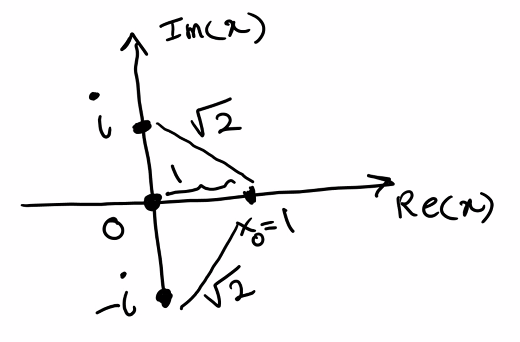
\includegraphics[width = 0.7 \textwidth]{image2.png}

$y(x) = \sum_{n = 0}^{\infty} a_n (x-1)^n$

$\rho = 1$ is the lower bound estimate. $\rho$ is the radius of convergence. Imagine a circle of radius 1 (as it's the distance to the closest singular point)

\subsubsection{An Example}

$$x^2 y'' + \alpha x y' + \beta y = 0$$

$r_1, r_2$ are two positive roots

$$y = C_1 x^{r_1} + C_2 x^{r_2}$$

$x_0 = 0$ is a singular point

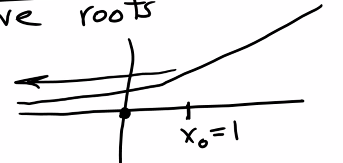
\includegraphics[width = 0.4 \textwidth]{image3.png}

Radius of convergence is infinite. This is a rare case. 

\section{Frobenius Series}

EX: 

$$ 6x^2 (1+x) y'' + 5xy' - y = 0$$

$P(x) = 6x^2 (1+x)$, $Q(x) = 5x$, $R(x) = -1$

Singular points are $x = 0$ and $x = -1$. 

For $x = 0$, let's find if it's irregular or regular:

$\lim_{x \to 0} \frac{Q(x)}{P(x)}(x - x_0) = \lim_{x \to 0} \frac{5x}{6x^2 (1+x)} x = \frac{5}{6} = p_0$

$\lim_{x \to 0} \frac{-1}{6x^2 (1+x)} x^2 = \frac{-1}{6} = q_0$

Therefore $x_0 = 0$ is a regular singular point. 

$$(x - x_0)^2 y'' + \frac{5}{6} (x - x_0) y' - \frac{1}{6} y = 0$$

This is for $x_0 = 0$. Hence, $x^2 y'' + \frac{5}{6} x y' - \frac{1}{6} y = 0$. 

\hfill \break 

Corresponding Cauchy-Euler equation:

$y = x^r$ and therefore $\left[ 6r(r-1) + 5r - 1 \right] x^r = 0$. 

Hence $6r^2 - r - 1 = 0 \longrightarrow r_{1,2} = \frac{1 \pm \sqrt{1+24}}{12} \longrightarrow r_{1,2} = \frac{1}{2}, \frac{-1}{3}$

\hfill \break 

Frobenius Series Solution about $x = 0$:

$$y(x) = x^2 \sum_{n = 0}^{\infty} a_n x^n = \sum_{n = 0}^{\infty} a_n x^{n+r}$$

$$y' = \sum_{n = 0}^{\infty} a_n (n+r) x^{n+r-1}$$

$$y'' = \sum_{n = 0}^{\infty} a_n (n+r)(n+r-1) x^{n+r-2}$$

Now, we only need to replace $y, y', y''$ in the ODE:

$$6x^2(1+x) y'' + 5xy' - y = 0$$

$$6x^2 y'' + 6x^3 y'' + 5xy' - y = 0$$

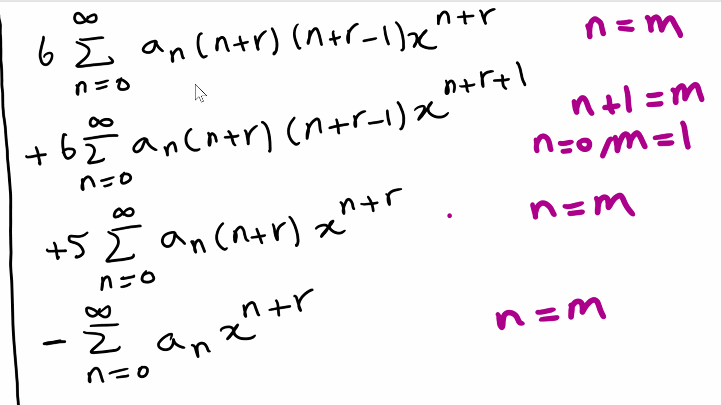
\includegraphics[width = 0.95 \textwidth]{image4.png}

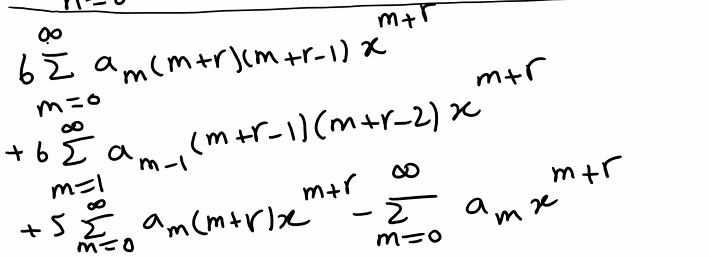
\includegraphics[width = 0.95 \textwidth]{image5.png}

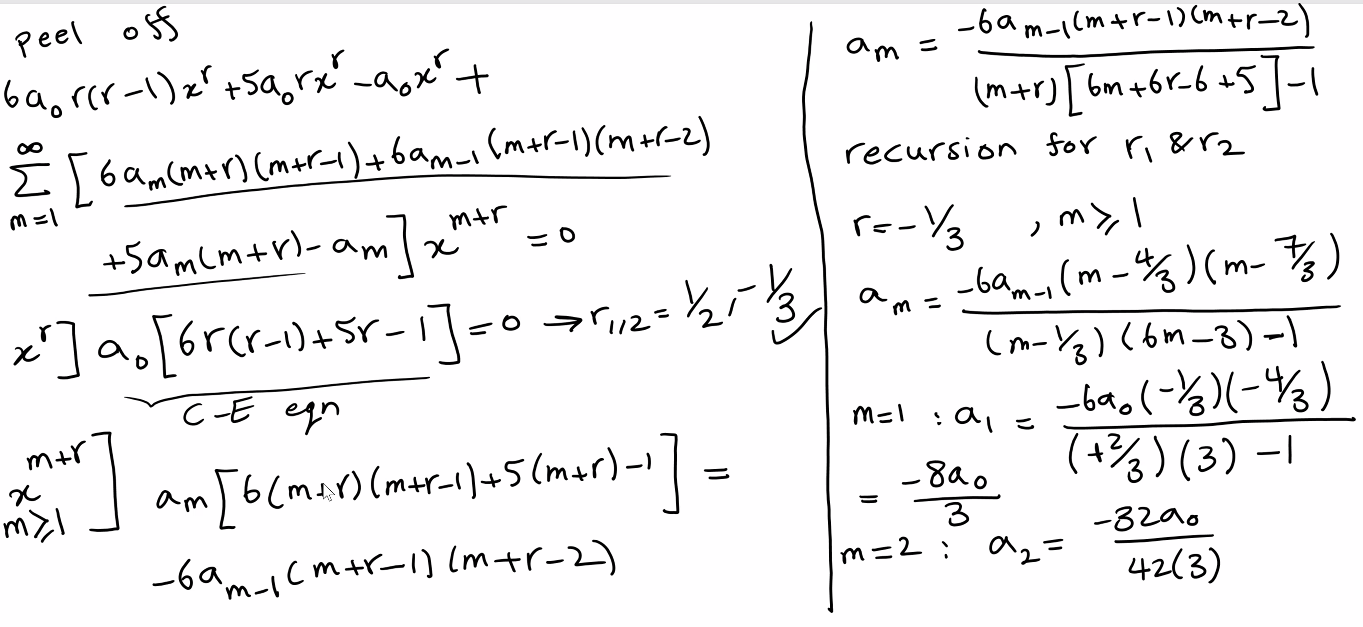
\includegraphics[width = 0.95 \textwidth]{image6.png}

$$y_1(x) = a_0 x^{\frac{-1}{3}} \left[ 1- \frac{8}{3} x - \frac{32}{3(42)} x^2 + ... \right]$$

$r = \frac{1}{2}$: If we follow the same steps, we get 

$y_2(x) = \underbrace{a_0}_{\text{A different } a_0} x^{\frac{1}{2}} \left[ 1 + \frac{3}{22} x - \frac{22}{22.68}x^2 + ... \right]$

Hence the general solution is $y = C_1 y_1 (x) + C_2 y_2 (x)$

\subsubsection{Convergence: ratio test}

$$\sum_{m = 0}^\infty C_m: \lim_{m \to \infty} | \frac{C_{m+1}}{C_m} | < 1$$

$$y(x) = \sum_{m = 0}^\infty a_m x^{m+r}$$

Ratio test:

$$\lim_{m \to \infty} | \frac{a_{m+1} x^{m+r+1}}{a_m x^{m+r}} | = |x| \lim_{m \to \infty} | \frac{a_{m=1}}{a_m}$$

For this example:

$$ |x| \lim_{m \to \infty} | \frac{a_{m=1}}{a_m}, a_m = \frac{-6 a_{m-1} (m+r-1) (m+r-2)}{(m+r) (6m + 6r - 1) - 1}$$

$$ |x| \lim_{m \to \infty}  \frac{-6 a_{m-1} (m+r-1) (m+r-2)}{(m+r) (6m + 6r - 1) - 1} = |x| \cdot 1$$

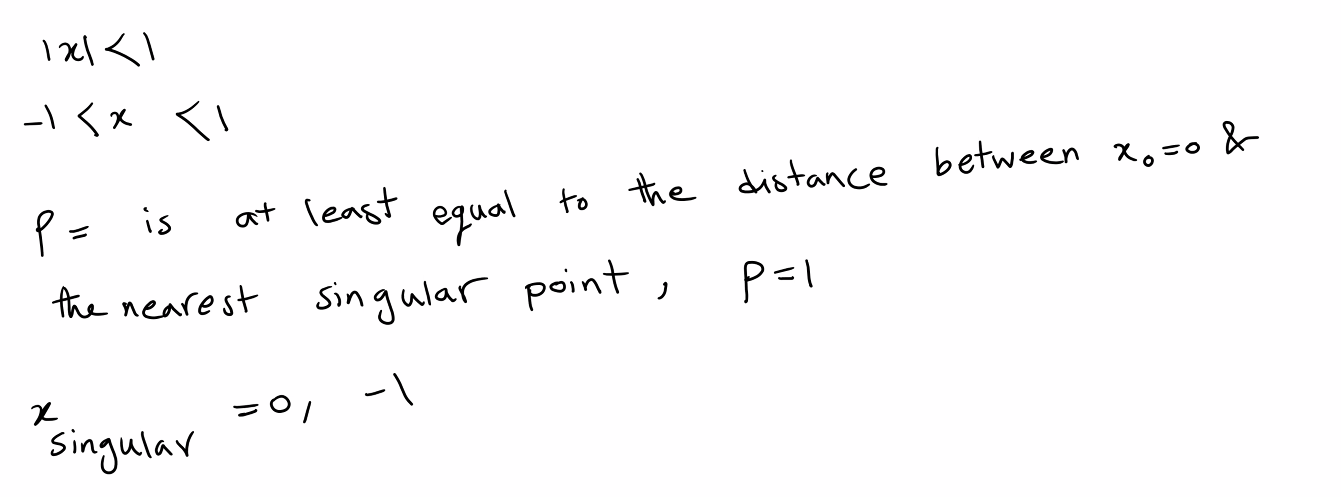
\includegraphics[width = 0.95 \textwidth]{image7.png}

\chapter{Lecture 4}

\section{Introduction}

\subsection{Week 2:}

\begin{itemize}
    \item finish power series
    \item Bessel's function
    \item Intro to PDEs
\end{itemize}

\subsection{Week 3:}

\begin{itemize}
    \item Fourier series and separation of variables
    \item Heat equations
    \item Wave equations
    \item Laplace equations
\end{itemize}

\subsection{Week 4:}

\begin{itemize}
    \item Boundary value problems and Sturm-Louiville Theory
    \item Eigenfunctions and eigenvalues
    \item Sturm-Louisvill theory for BVP
    \item Non-homogenous boundary value problems
\end{itemize}

\subsection{Week 5:}

\begin{itemize}
    \item Numerical methods for solving PDEs
\end{itemize}

\section{Recap of Previous Week}

What we're covering next was partly covered in previous lectures by Parisa:

\hfill

Series Solutions near a regular singular point (RSP)

$$ P(x) y'' + Q(x) y' + R(x)y = 0$$

We consider an expansion about a regular singular point $x_0$ of the ODE. 

Next, we take the limits:

$$\lim_{x \to x_0} (x - x_0) \frac{Q(x)}{P(x)} = p_0$$

$$\lim_{x \to x_0} (x - x_0)^2 \frac{R(x)}{P(x)} = q_0$$

When these two limits exist and are finite, then this leads to the following. We divide $ P(x) y'' + Q(x) y' + R(x)y = 0$ by $P(x)$ and multiply it by $(x - x_0)^2$:

$$(x-x_0)^2 y'' + (x - x_0) \underbrace{\left\{(x - x_0) \frac{Q(x)}{P(x)} \right\}}_{p(x) = p_0 + p_1 (x - x_0) + ...} y' + \underbrace{\left\{ (x - x_0)^2 \frac{R(x)}{P(x)} \right\}}_{q(x) = q_0 + q_1 (x - x_0) + ...} y = 0$$


$$(x - x_0)^2 + p_0 (x - x_0) y' + q_0 y = 0$$

is the C-E equation. This equation has a solution of the following format:

$$y_0(x) = (x - x_0)^r$$

To include the effect of the neglected terms, we modify the above solution:
$$y(x) = \underbrace{(x - x_0)^r}_{\text{C-E solution}} \sum_{n = 0}^{\infty} \underbrace{a_n (x - x_0)^n}_{\text{The solution}}$$


with $a_0 \neq 0$. (2) is the modified equation for $y_0(x) = (x - x_0)^r$ and is  Frobenius series. 

\subsection{Solution procedure}

\begin{enumerate}
    \item Find values of r
    \item Find the recursive relation for n
    \item Find the radius of convergene for $\sum_{n = 0}^{\infty} a_n (x - x_0)^{n +r}$
\end{enumerate}

\subsection{Example 1}

$$Ly = 2x^2 y'' - x y' + (1-x)y = 0$$

Singular point here is when $x_0 = 0$

Again, to test if it is a singular point, we take the limits. 

$$p_0 = \lim_{x \to 0} \frac{-x}{2x^2} x = \frac{-1}{2}$$

Similarly, we check $q_0$:

$$q_0 = \lim_{x \to 0} \frac{(1-x)}{2x^2} x^2 = \frac{1}{2} = q_0$$

Hence, the singular point is a RSP. 

$$\Rightarrow y(x) = x^r \sum_{n = 0}^\infty a_n x^n$$

Step 1: Find values of r

Characteristic equation: $r(r-1) + p_0 r + q_0 = 0$

This becomes $r(r-1) - \frac{r}{2} + \frac{1}{2} = 0 \Rightarrow r^2 - \frac{3}{2} r + \frac{1}{2} = 0$

Hence, $r = 1$ and $r = \frac{1}{2}$ are roots of the indicial equation. 

$$y_0 = c_1 x + c_2 x^{\frac{1}{2}}$$

Now, we go to step 2: Find the recursive relation for $n$. 

Take the first and second derivative of the summation (that we've used before) and sub into the equation. 

$$2\sum_{n = 0}^{\infty} a_n (n+r)(n+r-1) x^{n+r} - \sum_{n = 0}^{\infty} a_n (n+r) x^{n+r} + \sum_{n = 0}^\infty a_n x^{n+r} - \sum_{n = 0}^\infty a_n x^{n+r+1} = 0$$

Changing index:

$$2\sum_{n = 0}^{\infty} a_n (n+r)(n+r-1) x^{n+r} - \sum_{n = 0}^{\infty} a_n (n+r) x^{n+r} + \sum_{n = 0}^\infty a_n x^{n+r} - \underbrace{\sum_{n = 0}^\infty a_n x^{n+r+1}}_{m = n+1} = 0$$

All others are $m = n$. 

With that, we get the following:

$$2\sum_{n = 0}^{\infty} a_n (n+r)(n+r-1) x^{n+r} - \sum_{n = 0}^{\infty} a_n (n+r) x^{n+r} + \sum_{n = 0}^\infty a_n x^{n+r} - \sum_{n = 1}^\infty a_{n-1} x^{n+r}$$
(Removing $=0$ due to space)

Peeling off the first terms ($n=0$), we end up with the following sum:

$$\underbrace{2 a_n r(r-1)x^r - a_0 r x^r + a_0 x^r}_{ = a_0 x^r \left( 2r^2 - 3r + 1 \right)} \longrightarrow ...$$
$$\hookrightarrow + \sum_{n = 1}^\infty \left[ 2 a_n (n+r) (n+r-1) - a_n (n+r) + a_{n-1} \right] x^{n+r} = 0$$

Hence, $a_n = \frac{a_{n-1}}{(n+r)(2(n+r)-3) + 1}$ is the recursive relation for r values

Finding the recursive relation for $r_1$ and $r_1$:

$$r_1 \Rightarrow a_n = \frac{a_{n-1}}{(n+1)(2(n+1)-3)+1} = \frac{1_{n-1}}{2n^2 + n}$$

$n = 1: a_1 = \frac{a_0}{3}; n = 2: a_2 = \frac{a_1}{10} = \frac{a_0}{30}; n = 3: a_3 = \frac{a_2}{21} = \frac{a_0}{630}$

Therefore:

$$y(x) = a_0 x^1 (1 + \frac{x}{3} + \frac{x^2}{30} + \frac{x^3}{630} + ...)$$

Next, for $r_1 = \frac{1}{2}$:

$$a_n  =\frac{a_{n-1}}{(n + \frac{1}{2} (2n+1-3) + 1} = \frac{a_{n-1}}{2(n + \frac{1}{2})(n-1) + 1}$$

$n = 1: a_1 = \frac{a_0}{1}; n = 2:  a_2 = \frac{a_1}{6} = \frac{a_0}{6}; n = 3: a_3 = \frac{a_0}{90}$

So, we have the following:

$$y_2(x) = a_0 x^{\frac{1}{2}} \left[ 1 + x + \frac{x^2}{6} + \frac{x^3}{90} + ... \right]$$

Now, onto step 3:

Find the radius of convergence. 

To find the radius of covergence, we use the ratio test:

$$\lim_{n \to \infty} | \frac{a_n x^n}{a_{n-1}x^{n-1}}|$$

$$ = \lim_{n \to \infty} | \frac{a_{n-1} x^n}{(n+r) (2(n+r)-3) + 1} \frac{1}{a_{n-1} x^{n-1}} |$$

\textbf{The above is not correct. Why?}

$$\lim_{n \to \infty} |x| |\frac{1}{(n+r) (2(n+r)-3)+1}| = 0$$

$\Rightarrow p = \infty$ for all $x$ values

Final solution:

$$y(x) = y_1(x) + y_2(x)$$

$$y(x) = C_1 x \left(1 + \frac{x}{3} + \frac{x^2}{30} + \frac{x^3}{630} + ... \right) + C_2 x^\frac{1}{2} \left(1+x+\frac{x^2}{6} + \frac{x^3}{90} + ... \right)$$


\section{Bessel's equation}

Applications: PDEs on circular / cylindrical domain. 

e.g. heating and cooling in circular / cylindrical geometries, i.e. pipes and heat exchangers. 

\hfill

The equation format:
\begin{equation}
    \label{Bessel's Equation}
    Ly = x^2 y'' + xy' + \left(x^2 - \nu^2 \right) y = 0
\end{equation}

$\nu$ is a constant and specifies the order of the equation. 

$x_0 = 0$ is a regular singular point, since $\lim_{x \to 0} \frac{x}{x^2} (x) = 0 = p_0$ and $\lim_{x \to 0} \frac{x^2 - \nu^2}{x^2}(x^2) = - \nu^2 = q_0$

\subsection{Step 1: Finding the $r$ values}

The characteristic equation is:

$$r(r-1) + p_0 r + q_0 = 0$$

$$r(r-1) + r - \nu^2 = 0 \Rightarrow r = \pm \nu$$

\subsection{Step 2: Frobenius part -- Finding recursive relation}

$$y = \sum_{n = 0}^\infty a_n x^{n+r}$$

$$y' = \sum_{n =0}^{\infty} a_n (n+r)x^{n+r-1}$$

$$y'' = \sum_{n=0}^{\infty} a_n (n+r) (n+r-1) x^{n+r-2}$$

Substituting into the equation, we get the following:

$$Ly = x^2 y'' + xy' + \left(x^2 - \nu^2 \right) y = 0$$

$$Ly = x^2 \sum_{n=0}^{\infty} a_n (n+r) (n+r-1) x^{n+r-2} \rightarrow ...$$

$$ \hookrightarrow + x\sum_{n =0}^{\infty} a_n (n+r)x^{n+r-1} \rightarrow ...$$
$$ \hookrightarrow + \left(x^2 - \nu^2 \right) \sum_{n = 0}^\infty a_n x^{n+r} = 0$$

Shifting index:

$$Ly = x^2 y'' + xy' + \left(x^2 - \nu^2 \right) y = 0$$

$$Ly = x^2 \sum_{n=0}^{\infty} a_n (n+r) (n+r-1) x^{n+r-2} \rightarrow ...$$

$$ \hookrightarrow + x\sum_{n =0}^{\infty} a_n (n+r)x^{n+r-1} \rightarrow ...$$
$$ \hookrightarrow + \underbrace{x^2\sum_{n = 0}^\infty a_n x^{n+r+2}}_{m = n+2} - \nu^2\sum_{n = 0}^\infty a_n x^{n+r} = 0$$

Hence, we get the following:

$$Ly = \sum_{n = 0}^\infty a_n (n+r)(n+r-1) x^{n+r} + \sum_{n=0}^\infty a_n (n+r) x^{n+r} + \sum_{n = 2}^\infty a_{n-2} x^{n+r}$$

Next, we peel off the first two terms to match the summation. 

$$a_0 (r(r-1) + r - \nu^2) x^r + a_1 ((1+r) r + (1+r) - \nu^2) x^{r+1} \rightarrow ... $$
$$ \hookrightarrow + \sum_{n = 2}^\infty a_n \left[ a_n \left( (n+r)^2 - \nu^2 \right) + a_{n-2} \right] x^{n+r} = 0$$

$$a_0 x^r (r^2 - \nu^2) + a_1 x^{r+1} \left((r+1)^2 - \nu^2 \right)  + \sum_{n = 2}^\infty a_n \left[ a_n \left( (n+r)^2 - \nu^2 \right) + a_{n-2} \right] x^{n+r} = 0$$


\chapter{Lecture 5}
\graphicspath{{./Lecture5/}}

\section{Bessel's Equation, continued from last class}

$$a_0 (r(r-1) + r - \nu^2) x^r + a_1 \left((1+r)r + (1+r) - \nu^2 \right) x^{r+1} + \sum_{n = 2}^\infty a_n \left(... \right) x^{n+r} = 0$$

We can use linear independency. This means that the set of the coefficients of all powers of $x$ must be zero.

The following is found from the characteristic equation:

$$x^r | a_0 (r^2 - \nu^2) = 0 \longrightarrow r = \pm \nu \text{ }\& \text{ } a_0 \neq 0$$

$$x^{r+1} | a_1 \left(r^2 + 2r + 1 - \nu^2 \right) = 0 \underbrace{\longrightarrow}_{\nu^2 - r^2} a_1 (2 \nu + 1) = 0$$

$$\hookrightarrow \left\{ \begin{matrix} \nu = \pm \frac{1}{2} &  \& & q \neq 0 \\ \nu \neq \pm \frac{1}{2} & \& & q = 0 \end{matrix} \right.$$

$$x^{n+r} | \left((n+r) (n+r-1) + (n+r) - \nu^2 \right) a_n + a_{n-2} = 0 \longrightarrow n \geq 2$$

$$(**)\text{ } a_n = \frac{-a_{n-2}}{(n+r)^2 - \nu^2}$$

Find the recursive relation for $r = \pm \nu$:

$r_1 = \nu$: $a_n = \frac{-a_{n-2}}{(n+\nu)^2 - \nu^2} = \frac{-a_{n-2}}{n(n + 2 \nu)}$,  $(n \geq 2)$

*writing down $a_2$, $a_3$, and $a_4$*

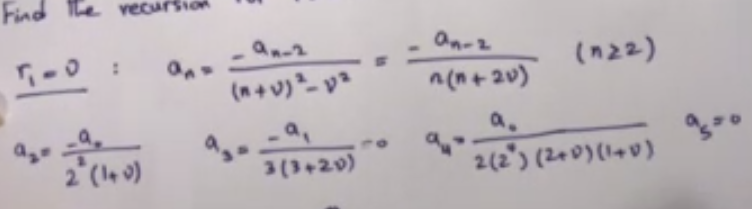
\includegraphics[width = 0.8 \textwidth]{image2.png}

\hfill

$\Rightarrow a_{2m} = \frac{(-)^m a_0}{m! 2^{2m} (1 + \nu) (2 + \nu) ... (m + \nu)}$

$$y_1(x) = a_0 x^{\nu} \sum_{m = 0}^\infty \frac{(-1)^m x^{2m}}{m! 2^{2m} (1 + \nu)(2 + \nu) ... (m + \nu)}$$

Now, for $r_1 = \nu$:

$$a_n = \frac{-1_{n-1}}{(n - \nu)^2 - \nu^2} = -\frac{a_{n-2}}{n(n - 2 \nu)}; n \geq 2$$

$$a_2 = \frac{-a_0}{2(2-2\nu)} = \frac{-a_0}{2(2)(1-\nu)}$$

$$a_4 = \frac{-a_2}{4(4-2\nu)} = \frac{a_0}{4(2)(2-\nu)(2^2)(1 - \nu)}$$

$$a_6 = \frac{-a_4}{6(6 - 2 \nu)} = \frac{-a_0}{6(2)(3-\nu)2^5 (2 - \nu) (1 - \nu)}$$

Note that $a_1 = a_3 = a_5 .... = 0$

$$\Rightarrow a_{2m} = \frac{(-1)^m a_0}{m! 2^{2m} (1-\nu)(2 - \nu) (3 - \nu) ... (m - \nu)}$$

$$ y_2(x) = a_0 x^{-\nu} \sum_{m = 0}^\infty \frac{(-1)^m a_0}{m! 2^{2m} (1-\nu)(2 - \nu) ... (m - \nu)}$$

Finally, $y(x)$ is a linear combination of 2 solutions:

$$y(x) = C_1 x^{\nu} \underbrace{\sum_{m = 0}^\infty \frac{(-1)^m (x/2)^{2m}}{m (1 + \nu)(2 + \nu) ... (m + \nu)}}_{J_\nu \text{: Bessel Functions of the first kind}} + C_2 \underbrace{x^{-\nu} \sum_{m = 0}^\infty \frac{(-1)^m a_0}{m! 2^{2m} (1-\nu)(2 - \nu) ... (m - \nu)}}_{Y_\nu \text{: Bessel function of the second kind}}$$

We will be given this in the formula sheet. Note that $C_1$ and $C_2$ are not included in $J_\nu$ and $Y_\nu$.

For $\nu \neq \pm \frac{1}{2}$: As $x \to  0$, $J_\nu \to 0$ and $x \to  0$, $Y_\nu \to \infty$

What happens when $\nu = 0$?

$$x^r | a_0 (r^2 - \nu^2) = 0 \rightarrow r = \pm \nu, a_0 \neq 0$$

Two solutions are the same. Therefore, $r_{1,2} = 0$


Then, $J_\nu(x) = C_1 x^0 \sum_{m = 0}^\infty \frac{(-1)^m}{(m!)^2} \left(\frac{x}{2} \right)^{2m}$

How about $Y_\nu (x)$?

Similar to Euler's equation (Refer to section 5.4 of the textbook), the second solution for repeated roots is:

$$y_2 (x) = y_1(x) \ln(x) + x^{r_1} \sum_{n = 1}^\infty a_n ' (r_1) x^n$$

where $a_n ' (r_1) = \left. \frac{d a_1}{dr} \right|_{r = r_1}$

According to this formula, $y_0 = J_0 (x) \ln(x) + x^{0} \sum_{n = 1}^\infty a_n' (0) x^n$ (***)

The recursion for this case (**) is found to be 

$$a_{2m} (r) = - \frac{a_{2m-2}}{(r + 2m)^2}, m = 1,2,3,...$$

$$a_{2m}(r) = \frac{(-1)^m a_0}{(r+2)^2 .... (r + 2m)^2}$$

$$a_{2m}' (r) = -2 \left( \frac{1}{r+2} + \frac{1}{r+4} + ... + \frac{1}{r + 2m} \right) a_{2m} (r)$$

$$a_{2m}' (0) = -2 \left( \frac{1}{2} + \frac{1}{4} + .... + \frac{1}{2m} \right) a_{2m}(0) = - \left(\frac{1}{2} + \frac{1}{4} + .... + \frac{1}{2m} \right) \frac{(-1)^m a_0}{2^{2m} (m!)^2} $$

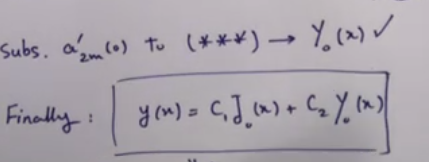
\includegraphics[width = 0.8 \textwidth]{image3.png}

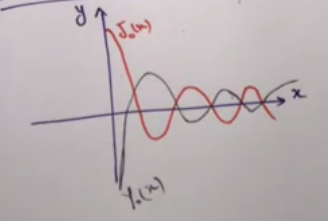
\includegraphics[width = 0.8 \textwidth]{image4.png}

As $x \to 0$, $y_0 (x) \to - \infty$, i.e. if the solution, $y(x)$, is finite at zero, then $C_2 = 0$

\section{Bessel Equation of Order of $\pm \frac{1}{2}$}

$$Ly = x^2 y'' + xy' + (x^2 - \frac{1}{4} )y = 0$$

$$x^r | a_0 (r^2 - \nu^2) = 0 \longrightarrow a_0 \neq 0 \text{ and } r = \pm \nu$$

For $\nu = \frac{1}{2} \Rightarrow r = \pm \frac{1}{2}$

$$x^{r+1} | a_1 (r^2 + 2r + 1 - \nu^2) = 0 \Rightarrow a_1 (1 \pm 2 \nu) = 0$$

If $\nu = \pm \frac{1}{2}$, $a_1$ is arbitrary

$$x^{m+r} | -a_m (r^2 + 2r + 1 - \nu^2) = a_{m=2} \Rightarrow a_m = \frac{-a_{m-2}}{(m+r)^2 - \nu^2}$$

For $\nu \pm \frac{1}{2}, a_m = \frac{-a_{m-2}}{(m+\frac{1}{2})^2 - \frac{1}{4}} = \frac{-a_{m-2}}{m(m+1)}$

Let $r_1 = \frac{1}{2}$: $a_1 (1 + 2 (\frac{1}{2})) = 0 \Rightarrow a_1 = 0$

$a_2 = - \frac{a_0}{2(3)}$, $a_4 = \frac{-a_2}{3(4)} = \frac{a_0}{5!}$

Therefore:

$$y_1 (x) = a_0 x^{\frac{1}{2}} \underbrace{\left(1 - \frac{x^2}{3!} + \frac{x^4}{5!} + ... \right) \frac{x}{x}}_{\text{Taylor series for } \sin(x)}$$

$$y_1(x) = a_0 x^{- \frac{1}{2}} \sin(x)$$

let $r_2 = \frac{-1}{2}$: $a_1 (1 - 2 \frac{1}{2}) = 0 \Rightarrow$ $a_1$ is arbitrary. it could be another solution.


for this case, $a_m = \frac{-a_{m - 2}}{(m = \frac{1}{2})^2 - \frac{1}{4}} = \frac{-a_{m - 2}}{m(m-1)}$

$a_2 = \frac{-a_0}{2(1)}$, $a_4 = \frac{-a_2}{4(3)} = \frac{a_0}{4!}$

$$\Rightarrow y_x(x) = a_0 x^{\frac{-1}{2}} \left(1 - \frac{x^2}{2!} + \frac{x^4}{4!} - ... \right) = a_0 x^{- \frac{1}{2}} \cos(x)$$

Let's check for $a_1 \neq 0$:

$a_3 = \frac{-a_1}{3 \cdot 2}$, $a_5 = \frac{-a_3}{5 \cdot 4} = \frac{a_1}{5!}$

$y_3 (x) = a_1 x^{- \frac{1}{2}} \sin(x)$. But this doesn't give us another solution -- This is the same as $y_1$; they are not independent. 

Hence we write the final solution as:

$$y(x) = a_0 x^{\frac{-1}{2}} \cos(x) + a_1 x^{\frac{-1}{2}} \sin(x)$$

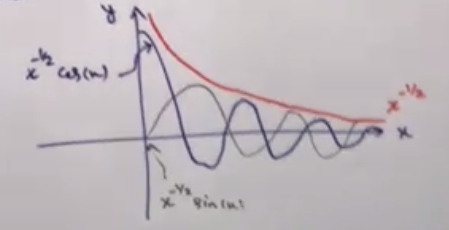
\includegraphics[width = 0.9 \textwidth]{image5.png}

\textbf{End of series functions}

\section{Introduction to PDE Classification}

What is a PDE?

A differential equation that includes partial derivatives with respect to all independent variables. 

$u(x,t) \longrightarrow$ PDEs include $\frac{\partial u}{\partial t}$, $\frac{\partial u}{\partial x}$, $\frac{\partial^2 u}{\partial x \partial t}$, $\frac{\partial^2 u}{\partial x^2}$, ...

\begin{itemize}
    \item Heat equation
    \item Wave equation
    \item Laplace equation
\end{itemize}

\chapter{Lecture 6}
\graphicspath{{./Lecture6/}}

\section{Recap of Frobenius Series Solutions}

Assume $x_0$ is a singular point of the ODE of the form:

$$P(x) y'' + Q(x) y' + R(x) y = 0$$

If $x_0$ is a regular singular point,

$$\lim_{x \to x_0} \frac{Q(x)}{P(x)} x = p_0$$

and

$$\lim_{x \to x_0} \frac{R(x)}{P(x)} x^2 = q_0$$

The characteristic equation is:

$$r(r-1) + p_0 r + q_0 = 0 \longrightarrow \text{2 roots: } r_1, r_2$$

For $r_1$, we get $y_1(x) = |x|^{r_1} \left( 1 + \sum_{n= 1}^{\infty} a_n x^n \right) = \sum_{n = 0}^\infty a_n x^{n + r_1}$

$a_n$ is found from a recursion by substitution into the ODE. $a_0$ is arbitrary. 

\hfill

1) If $r_1 - r_2 \neq 0$ and $r_1 - r_2 \neq N$ (N is an integer), then:

$$y_2 = |x|^{r_2} \left(1 + \sum_{n = 1}^\infty a_n x^n \right) = \sum_{n = 0}^\infty a_n x^{n + r_2}$$

2) If $r_1 = r_2$:

$$y_2(c) = y_1 (x) \ln(x) + |x| ^{r_1} \sum_{n = 1}^\infty C_n x^n = y_x(x) \ln(x) + \sum_{n = 1}^\infty C_n x^{n + r_1}$$

Note that $x > 0$. 

\hfill

Where $c_n = a_n ' = \left. \frac{d a_n}{dr} \right|_{r = r_1}$


Note 1: What happens of $r_1$ and $r_2$ are complex?

If they are, the form of $y_2$ in 1) (that we discussed), and $y_1$ are still valid; we just need to convert complex valued to real valued solutions. Needs lots of algebra. 

Note 2: A summary of these solutions is given in the formula sheet for the exam. 

Note 3: The general solution is in the following format:

$$y(x) = C_1 y_1(x) + C_2 y_2(x)$$

\hfill

\section{PDEs}

Continued from last class's notes. 

\subsubsection{Heat equation / diffusion equation}

$$\frac{\partial u}{\partial t} = k \frac{\partial^2 u}{\partial x^2} + k \left(\frac{\partial^2 u}{\partial y^2} + \frac{\partial^2 u}{\partial z^2} \right)$$

Applications: heat flows, diffusion of chemical substances

\subsubsection{Wave equation}

$$\frac{\partial^2 u}{\partial t^2} = C^2 \frac{\partial^2 u}{\partial x^2} + C^2 \left(\frac{\partial^2 u}{\partial y^2} + \frac{\partial^2 u}{\partial z^2}\right)$$

Applications: Vibrations, acoustics, solid mechanics

\subsubsection{Laplace's equation}

$$0 = \frac{\partial^2 u}{\partial z^2} + \frac{\partial^2 u}{\partial y^2}$$

Applications: Heat / wave equations in which there is a steady-state solution (eg potential flow, porous media flow)

\subsection{Classification of PDEs}

\hfill

ODEs: $f(x,u(x), u'(x)) = 0$. e.g. $u' = e^u$

\hfill

PDEs: $\underbrace{a(x,y) u_x + b(x,y) u_y = c(x,y) u}_{\text{First order, linear PDE}}$

\hfill

The solution to a PDE would look like a 2d surface: 

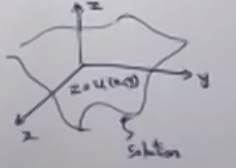
\includegraphics[width = 0.7 \textwidth]{image1.png}

Another example of a surface from WolframAlpha:

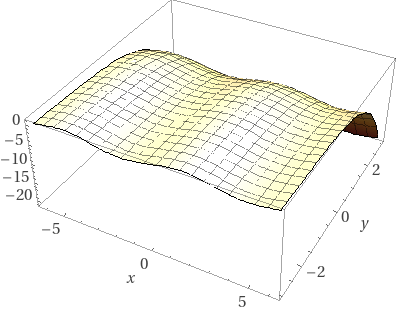
\includegraphics[width = 0.7 \textwidth]{image6.png}

\hfill

This course primarily focuses on second order linear PDEs. 
\begin{equation}
    A u_{xx} + 2 B u_{xy} + C u_{yy} + D u_x + E u_y + Fu = G
\end{equation}

$A,B,C,D,E,F,G$ can either be constants or functions of $(x,y)$.

The examples that we saw (heat equation, wave eq, etc) are all examples of the above (1). 

\hfill


If $G = 0$, the PDE is homogeneous. Else, it is non-homogeneous. 

To classify PDEs we use the analogy with corresponding quadratic surfaces:

$$AX^2 + BXY + CY^2 + DX + EY = K$$

To classify, we use the discriminant:

$$\Delta = B^2 - 4AC$$

It tells us either ellipse ($\Delta < 0$), hyperbola ($\Delta > 0$), or a parabola ($\Delta = 0$)

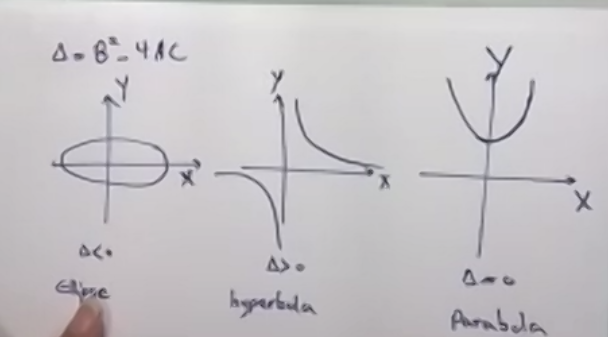
\includegraphics[width = 0.9 \textwidth]{image2.png}

$$\begin{matrix} 
\Delta & \text{Type} & \text{PDE} & \text{Note} \\ 
\Delta = 0 & \text{parabolic} & u_t = u_{xx} & \text{Heat eq} \\ 
\Delta < 0 & \text{elliptic} & u_{xx} + u_{yy} = 0 & \text{Laplace eq} \\
\Delta < 0 & \text{elliptic} & u_{xx} + u_{yy} = G & \text{Poisson's eq} \\
\Delta > 0 & \text{Hyperbolic} & u_{tt} = c^2 u_{xx} & \text{Wave eq}
\end{matrix}$$

\hfill

\subsection{Heat / Diffusion Equation}

Consider a rod of length $\Delta x$:

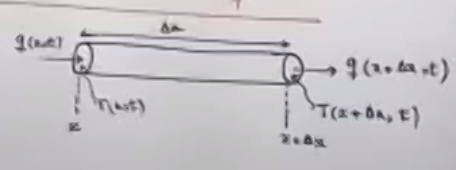
\includegraphics[width = 0.9 \textwidth]{image3.png}

\hfill

(The equations that are a bit blurry are the following, left to right and top to bottom: $q(x,t)$, $\Delta x$, $q(x + \Delta x, t)$, $T(x,t)$, $T(x + \Delta x, t)$, $x$, $x + \Delta x$)
\begin{itemize}
    \item $T(x,t)$: Temperature at $(x,t)$
    \item $q(x,t)$: The heat flux (heat energy per unit area)
    \item $C$: The specific heat capacity
    \item $\rho$: density of material
    \item $A$: The cross sectional area
\end{itemize}


Energy conservation: The increase in the thermal energy of the bar is equal to the (influx - outflux) of heat.  (Physical description, not mathematical description). 

Use variables: $C (T(x,t + \Delta t) - T(x,t)) \rho \Delta x A = (q (x,t) - q(x + \Delta x, t)) A \Delta t$

Divide by $\Delta t \cdot \Delta x$: 

$$\rho C \frac{T(x,t + \Delta t) - T(x,t)}{\Delta t} = \frac{q(x,t) - q(x,t + \Delta t)}{\Delta x}$$

As $\Delta t \to 0$ and $\Delta x \to 0$:

$$\rho C \frac{\partial T}{\partial t} = - \frac{\partial q}{\partial x}$$

The energy conservation equation is hence:

\begin{equation}
\label{energy conservation equation}
    \frac{\partial q}{\partial x} + \rho C \frac{\partial T}{\partial t} = 0
\end{equation}

In order to reduce the number of dependent variables, we need a constitutive equation between $q$ and $T$. Can we relate the heat flux to the temperature?

Yes. The heat transfer through conduction is formulated as:
\begin{equation}
\label{Fourier's Law}
\tag{Fourier's Law}
    q = -k \frac{\partial T}{\partial x}
\end{equation}

where $k$ is the thermal conductivity of the material. What does this tell us?

- Heat flux will flow from high temperature to low temperature. 

We can substitute \ref{Fourier's Law} in the energy conservation equation:

$$-k \frac{\partial^2 T}{\partial x^2} + \rho c \frac{\partial T}{\partial t} = 0$$

$$\hookrightarrow \frac{\partial T}{\partial t} = \alpha^2 \frac{\partial T}{\partial x^2}$$

Where $\alpha^2 = \frac{k}{\rho c}$ (diffusion coefficient). 

\subsection{Solving diffusion equations using separation of variables}

The initial boundary value problems, $u_t = \alpha^2 u_{xx}$, needs one initial condition (IC) and two boundary conditions (BC). 

Initial condition: $u(x,t = 0) = f(x)$ on the domain $0 < x < L$

\subsubsection{Boundary conditions}

(1) Dirichlet boundary conditions $u(0,t) = 0 = u(L,t)$ (i.e. same temperature on either side of the rod). Temperature is fixed: (see screenshot below). 

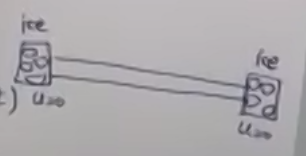
\includegraphics[width = 0.5 \textwidth]{image4.png}

(2) Neumann boundary conditions: $u_x (0,t) = 0 = u_x (L,t)$. i.e. insulation on either side of a rod. Temperature won't change with respect to $x$. 

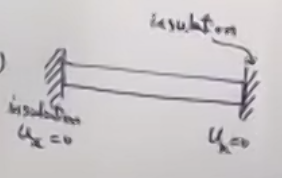
\includegraphics[width = 0.5 \textwidth]{image5.png}

(3): Mixed boundary conditions. $u(0,t) = 0$ and $u_x (L,t) = 0$

\subsubsection{Example 1}
\begin{center}
    $u_t = \alpha^2 u_{xx}$, $0 < x < L$, $t > 0$
\end{center}


Boundary conditions:

$$\begin{matrix} u(0,t) = 0 \\ u(L,t) = 0 \end{matrix}$$

Initial conditions: $$u(x,0) = f(x)$$

To solve, we use the method of separation of variables. We will do this next class. 


\chapter{Lecture 7}
\graphicspath{{./Lecture7/}}

\section{Boundary value Problems}

Is there a similar setup for BVPs/ Let's consider 3 different BVPs:
\begin{enumerate}
    \item P1: $y'' + \lambda y = 0$, for $x \in [0,L]$, with $y(0) = 0 = y(L)$
    \item P2: $y'' + \lambda y = 0$, for $x \in [0,L]$, with $y'(0) = 0 = y'(L)$
    \item P3: $y'' + \lambda y = 0$, for $x \in [0,L]$, with $y(0) = y(L)$ and $y'(0) = y'(L)$
\end{enumerate}

Any value of $\lambda$ for which P1 (P2 or P3) has a non-zero solution is called an \textbf{eigenvalue} of P1 (P2 or P3) and the corresponding solution is called and \textbf{eigenfunction} of P1 (P2 or P3).

Exercise: find the eigenvalues and eigenfunctions of problems P1, P2 and P3. 

\subsection{Solving BVP (P1,P2,P3)}

P1: \begin{center} $y'' + \lambda y = 0$, and $y(0) = 0 = y(L)$ \end{center}

$\lambda$: Eigenvalue. There are three categories that we have to investigate each time we solve such a problem:

\begin{enumerate}
    \item If $\lambda$ is negative ($\lambda < 0 $): 
    \begin{itemize}
        \item $\lambda = -\mu^2 \to y'' - \mu^2 y = 0$
        \item $r^2 - \mu^2 = 0 \to r_1 = \mu, r_2 = -\mu \longrightarrow y(x) = C_1 e^{\mu x} + C_2 e^{-\mu x}$
        \item Note that $\cosh(\mu x) = \frac{e^{\mu x} + e^{-\mu x}}{2} $ and $\sinh(\mu x) = \frac{e^{\mu x} - e^{-\mu x}}{2} \longrightarrow$
        \item $\hookrightarrow y(x) = A \sinh(\mu x) + B \cosh(\mu x)$
        \item 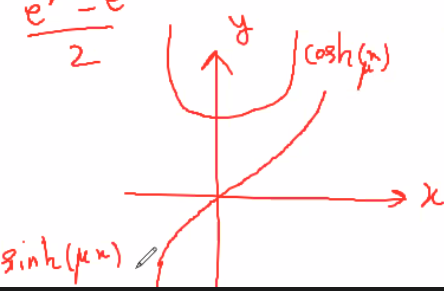
\includegraphics[width = 0.6 \textwidth]{image1.png}
        \item Note that we have the boundary conditions $y(0) = 0 \to B = 0$ and $y(L) = 0 \to A\sinh(\mu L) = 0$
        \item $\Rightarrow A = 0$ and $\Rightarrow y(x) = 0$ which is trivial
    \end{itemize}
    \item If $\lambda$ is zero: $y'' = 0 \longrightarrow y(x) = Ax + B$
    \begin{itemize}
        \item $y(0) = 0 \longrightarrow B = 0$
        \item $y(L) = 0 \longrightarrow AL = 0 \to A = 0 \to y(x) = 0$
        \item Therefore it's a trivial solution. 
    \end{itemize}
    \item If $\lambda > 0$: $\lambda = \mu^2 \to y'' + \mu^2 y = 0$
    \begin{itemize}
        \item $r^2 + \mu^2 = 0 \longrightarrow r = \pm i \mu$
        \item $y(x) = A \sin(\mu x) + B \cos(\mu x)$
        \item $y(0) = 0 \to B = 0$
        \item $y(L) = 0 \to A \sin(\mu L) = 0 \to \begin{matrix} A = 0 \text{(trivial)} \\ \sin(\mu L) = 0 \to \mu L = n \pi  \end{matrix} \text{ therefore } \mu = \frac{n \pi}{L}$
        \item Eigenvalue: $\lambda = \left(\frac{n \pi}{L} \right)^2$
        \item Eigenfunction: $y_n(x) = A_n \sin(\frac{n \pi}{L} x)$
    \end{itemize}
\end{enumerate}

\subsection{P2: $y'' + \lambda y = 0$}

$y'(0) = 0 = y'(L)$

$r^2 + \lambda = 0$
\begin{enumerate}
    \item If $\lambda > 0$, $\lambda = \mu^2$
    \begin{itemize}
        \item $r^2 + \mu^2 = 0 \longrightarrow r = \pm i \mu$
        \item $y(x) = A \sin(\mu x) + B \cos(\mu x)$
        \item Sub boundary conditions:
        \item $y'(0) = A = 0$ and $y'(L) = 0 \longrightarrow -B \mu \sin(\mu L) = 0$
        \item This gives us two solutions: $\begin{matrix} B = 0 \text{ which is trivial} \\ \underbrace{\sin(\mu L) = 0}_{\mu = \frac{n \pi}{L}} \end{matrix}$
        \item $\Rightarrow \lambda = \left( \frac{n \pi}{L}\right)^2$ is the eigenvalue
        \item $y_n (x) = B \cos \left( \frac{n \pi}{L} x \right)$ is the eigenfunction
        
    \end{itemize}
    \item If $\lambda < 0$: $\longrightarrow \lambda = -\mu^2$
    \begin{itemize}
        \item $r^2 - \mu^2 = 0 \longrightarrow r = \pm \mu \longrightarrow y(x) = C_1 e^{\mu x} + C_2 e^{-\mu x} \Rightarrow y(x) = A \sinh(\mu x) + B \cosh(\mu x)$
        \item Substituting the boundary conditions into $y(x) = A \sinh(\mu x) + B \cosh(\mu x)$, we get:
        \item $y'(0) = 0 \longrightarrow A = 0$
        \item $y'(L) = 0 \longrightarrow -\mu B \sinh (\mu L) = 0 \longrightarrow B = 0$ (which means that $y(x) = 0$ which is trivial)
    \end{itemize}
    \item If $\lambda = 0 \longrightarrow y'' = 0 \to y = Ax + B$
    \begin{itemize}
        \item $ y'(0) = 0 \to A = 0$ and $y'(L) = 0 \to A = 0$: $\longrightarrow$ $y(x) = B$
        \item $\lambda = 0$ is an eigenvalue $\longrightarrow y(x) = 1$ is the eigenfunction
        \item For P2 problems: eigenvalues are: $0, \frac{n^2 \pi^2}{L^2}$ and eigenfunctions are: $1, \cos\left(\frac{n \pi}{L} x \right)$
    \end{itemize}
\end{enumerate}

\subsection{P3: $y'' + \lambda y = 0$}

Periodic boundary conditions: $y(0) = y(L)$

\begin{enumerate}
    \item If $\lambda > 0$: $\lambda = \mu^2$
    \begin{itemize}
        \item $r = \pm \mu i \longrightarrow y(x) = A \sin(\mu x) + B \cos(\mu x)$
        \item $y(0) \ y(L) \longrightarrow B = A \sin(\mu L) + B \cos(\mu L)$
        \item $y'(0) = y'(L) \longrightarrow A \mu = A \mu \cos(\mu L) - B \mu \sin(\mu L)$
        \item 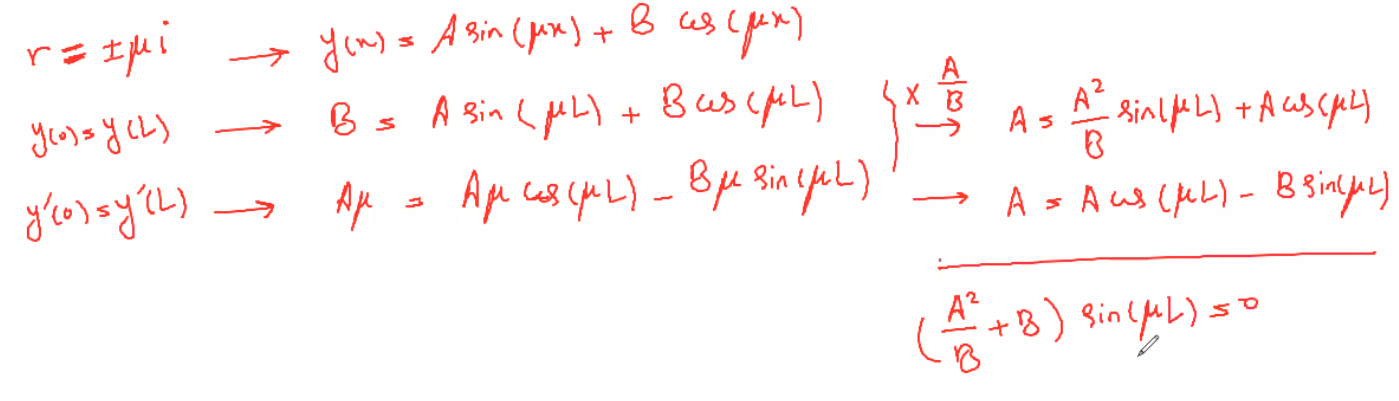
\includegraphics[width = 0.8 \textwidth]{image2.png}
        \item We get the last term by using the previous two terms (on the right) and cancelling out. 
        \item $\sin(\mu L) = 0 \to \mu L = n \pi$. $a \neq 0$ and $B \neq 0$ and therefore $\mu = \frac{n \pi}{L}$
        \item Eigenvalues: $\lambda = \left( \frac{n \pi}{L}\right)^2$
        \item Eigenfunction is $y_n (x) = A_n \sin(\frac{n \pi}{L} x) + B_n \cos(\frac{n \pi}{L} x)$
    \end{itemize}
    \item If $\lambda < 0$: $\lambda = -\mu^2$
    \begin{itemize}
        \item $y(x) = A \sinh(\mu x) + B \cosh(\mu x)$
        \item $y(0) = y(L) \longrightarrow B = A \sinh(\mu L) + B \cosh (\mu L)$
        \item $y'(0) = y'(L) \longrightarrow A = A \cosh(\mu L) - B \sinh(\mu L)$
        \item Multiplying $B = A \sinh(\mu L) + B \cosh (\mu L)$ by:
        \item 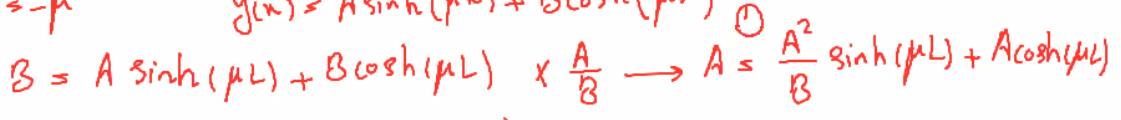
\includegraphics[width = 0.8 \textwidth]{image3.png}
        \item Okay this is going way too fast... screenshots it is. 
        \item 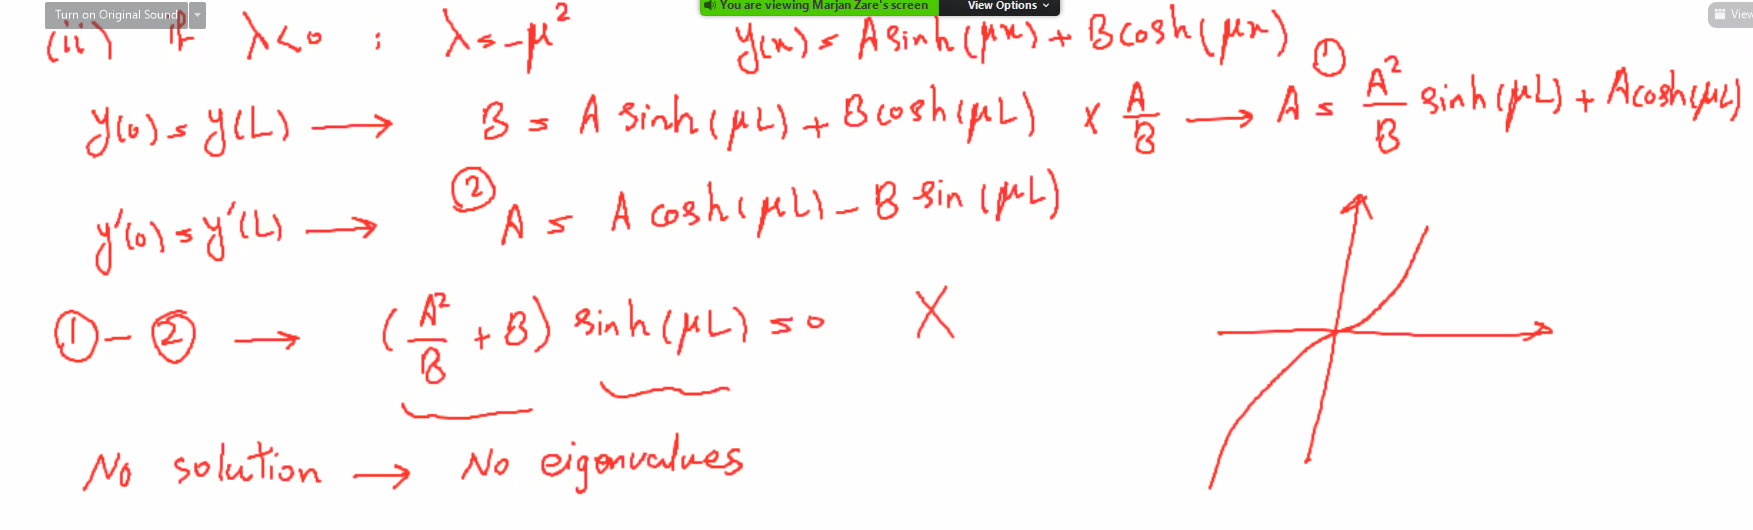
\includegraphics[width = 0.8 \textwidth]{image4.png}
    \end{itemize}
    \item $\lambda = 0$:
    \begin{itemize}
        \item View screenshot below. 
        \item 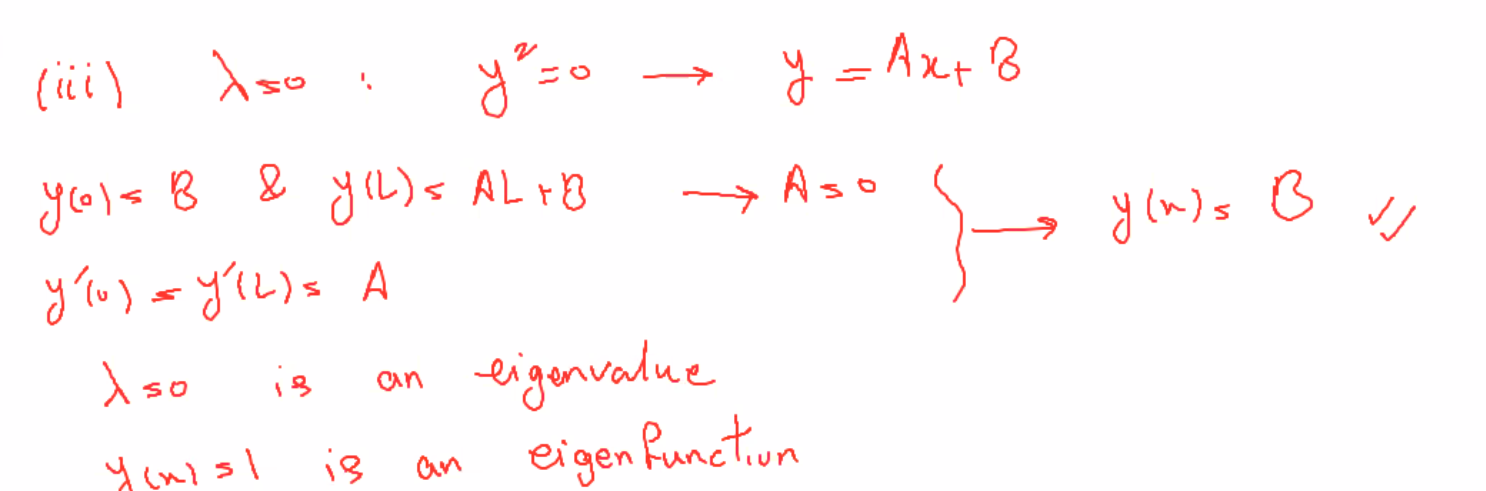
\includegraphics[width = 0.8 \textwidth]{image5.png}
    \end{itemize}
\end{enumerate}

\section{Fourier Series}

Fourier series arise in 3 different situations of relevance to this course:1.Simple boundary value problems, e.g. P1-P32.Partial differential equations that describe heat flow, waves and diffusion (more later).3.Some initial value problems with less simple periodic forcing, e.g. we are very unlikely to have exactly: $f(t) = F_0 \cos(\omega t)$, in any real system, but might have a periodic forcing function. \\ \hline

\hfill

For what follows, let the interval in P1-P3 be the interval $[a,b] = [-L, L]$. The key idea is that an arbitrary function, $f(t)$, defined on $[-L, L]$ can be represented in the following form:

\begin{equation}
    f(t) = \frac{a_0}{2} + \sum_{n = 1}^\infty a_n \cos(\frac{n \pi t}{L}) + \sum_{n = 1}^\infty b_n \sin(\frac{n \pi t}{L})
\end{equation}

Note that these are the eigenfunctions of problem P3. Outside of the interval,because each function above has period $2L$, the above series must converge to a periodic extension of $f(t)$ of period $2L$.

Two immediate questions:
\begin{enumerate}
    \item Can all functions $f(t)$ be represented in this way, i.e. which functions?
    \item How do we find the coefficients $a_n$ and $b_n$?
\end{enumerate}

\textbf{Definition}:If the series on the right-hand side of (1) converges to a function $f(t)$ then this is called the Fourier series of $f(t)$. 

\hfill

Comments:

Firstly, in order for $f(t)$ to have Fourier series representation(1), that is valid for all $t$ it is necessary that $f(t)$ is periodic, with period $2L$, i.e. $$f(t + 2L) = f(t) \text{     } \forall t$$

Secondly, suppose that $f(t)$ has a Fourier series representation (1). Then $a_n$ and $b_n$ are determined straightforwardly. See below for $a_n$:

\begin{enumerate}
    \item Multiply (1) by $\cos(\frac{m \pi t}{L})$
    \item Integrate both sides of the equation between $[-L, L]$:
\end{enumerate}

$$\int_{-L}^{L} f(t) \cos \frac{m \pi t}{L} d t=\int_{-L}^{L}\left(\frac{a_{0}}{2}+\sum_{n=1}^{\infty} a_{n} \cos \frac{n \pi t}{L}+\sum_{n=1}^{\infty} b_{n} \sin \frac{n \pi t}{L}\right) \cos \frac{m \pi t}{L} d t$$

Note that:

$$
\begin{array}{l}
\int_{-L}^{L} \cos \frac{n \pi t}{L} \cos \frac{m \pi t}{L} d t=\left\{\begin{array}{ll}
0 & m \neq n \\
L & m=n
\end{array}\right. \\
\int_{-L}^{L} \cos \frac{n \pi t}{L} \sin \frac{m \pi t}{L} d t=0 \\
\int_{-L}^{L} \sin \frac{n \pi t}{L} \sin \frac{m \pi t}{L} d t=\left\{\begin{array}{ll}
0 & m \neq n \\
L & m=n
\end{array}\right.
\end{array}
$$

Therefore, interchanging summation and integration:

$$
\begin{aligned}
\int_{-L}^{L} f(t) \cos \frac{m \pi t}{L} d t &=a_{m} \int_{-L}^{L} \cos \frac{m \pi t}{L} \cos \frac{m \pi t}{L} d t=a_{m} L \\
a_{m} &=\frac{1}{L} \int_{-L}^{L} f(t) \cos \frac{m \pi t}{L} d t
\end{aligned}
$$

For the coefficients $b_n$ a similar procedure is possible (exercise). 

Thus, we finally have:

$$
\begin{aligned}
a_{0} &=\frac{1}{L} \int_{-L}^{L} f(t) d t \\
a_{m} &=\frac{1}{L} \int_{-L}^{L} f(t) \cos \frac{m \pi t}{L} d t \quad m=1,2,3, \ldots \\
b_{m} &=\frac{1}{L} \int_{-L}^{L} f(t) \sin \frac{m \pi t}{L} d t \quad m=1,2,3, \ldots
\end{aligned}
$$

which are known as the \textbf{Euler-Fourier series}. 

\subsection{Example 1}
\begin{center}
    Assumer that the function $f(t)$, defined by $(t) = \left\{ \begin{matrix} t & -L \leq t < 0 \\ 0 & 0 \leq t < L \end{matrix} \right.$ with $ f(t + 2L) = f(t)$, has a fourier series. Sketch the function and find the fourier series. 
\end{center}

Solution:

$$f(t) = \frac{a_0}{2} + \sum_{n = 1}^\infty a_n \cos(\frac{n \pi t}{L}) + \sum_{n = 1}^\infty b_n \sin(\frac{n \pi t}{L})$$

$$a_0 = \frac{1}{L} \int_{-L}^L f(t) dt = \frac{1}{L} \int_{-L}^0 t dt = \frac{-L}{2}$$

$$a_n = \frac{1}{L} \int_{-L}^L f(t) \cos(\frac{n \pi t}{L}) dt = \frac{1}{L} \int_{-L}^0 t \cos (\frac{n \pi t}{L}) dt$$. 

Using integration by parts, with $u = t$ ($du = dt$) and $dv = \cos(\frac{n \pi t}{L}) dt$, with $v = \frac{L}{n \pi} \sin(\frac{n \pi t}{L})$, we get the following:

$$a_n = \frac{1}{L} \left[\frac{tL}{n \pi} \frac{\sin(n \pi t)}{L} \right|_{-L}^0 - \int_{-L}^{0} \frac{L}{n \pi} \frac{\sin(n \pi t}{L} dt$$

$$ = \frac{1}{n \pi} \left[ \frac{L}{n \pi} \cos(\frac{n \pi t}{L} |_{-L}^{0} \right] = \frac{L}{n^2 \pi^2} \left(1 - \cos(n \pi \right)$$

\chapter{Lecture 8}

\graphicspath{{./Lecture8/}}
\section{Introduction}

\begin{itemize}
    \item Midterm is on Tuesday, June 8th 12:30 to 2pm. 
    \item Send an email (on Canvas), and explain if you have difficulties regarding the exam including timezone differences. 
    \item Homeworks can be on Webwork. For the weeks that we have Webwork homework, it will be \textbf{instead} of written work. 
    \item It will be a mixture of webwork homework and written homework for the rest of the course; one week could we webwork and the next could be written. 
\end{itemize}

\section{Recap of last lecture}

We covered two categories last week:

We discussed eigenvalue problems, or boundary value problems, of (P1, P2, P3), which had the following form:

$$y'' + \lambda y = 0$$

with different boundary conditions:

\begin{itemize}
    \item P1 are Dirichlet boundary conditions (Fourier sine series)
    \item P2 are Neumann boundary conditions (Fourier cosine series)
    \item P3 are periodic boundary conditions (Mixture of Fourier sine and cosine series)
\end{itemize}

\subsection{Fourier series}

A periodic function on $(-L, L)$ and integrable can be written as 

$$f(t) = \frac{a_0}{2} + \sum_{n = 1}^\infty a_n \cos(\frac{n \pi t}{L}) + \sum_{n = 1}^\infty b_n \sin(\frac{n \pi t}{L})$$

$a_0$ can be found through the following formula:

$$a_0 = \frac{1}{L} \int_{-L}^L f(t) dt$$

$a_n$ can be found through

$$a_n = \frac{1}{L} \int_{-L}^{L} f(t) \cos(\frac{n \pi t}{L}) dt$$

And $b_n$ can be found from:

$$b_n = \frac{1}{L} \int_{-L}^L f(t) \sin(\frac{n \pi t}{L}) dt$$

\subsection{Example 1 (Continued from last class)}

$$f(t) = \begin{matrix} t & -L \leq t < 0 \\ 0 & 0 \leq t < L \end{matrix}, f(t + 2L) = f(t)$$

$a_0 = \frac{-L}{2}$; $a_n = \frac{L}{n^2 \pi^2} \left(1 - \cos(n \pi ) \right) = \frac{L}{n^2 \pi^2} \left(1 - (-1)^n \right)$ for $n \in {N}$

\hfill

$b_n = \frac{1}{L} \int_{-L}^L f(t) \sin(\frac{n \pi t}{L}) dt =  \frac{1}{L} \int_{-L}^0 t \sin(\frac{n \pi t}{L}) dt$

Using integration by parts, we get the following:

$b_n = \left. \frac{L}{n \pi}\left( \cos(n \pi) - \underbrace{\frac{\sin(n \pi)}{n \pi}}_{ = 0} \right) \right.$

$b_n = \frac{L}{n \pi} \cos(n \pi) = \frac{L}{n \pi} (-1)^n$ for $n \in N$

Substitute $(a_0, a_n, b_n)$ into the equation: 

$$f(t) = \frac{a_0}{2} + \sum_{n = 1}^\infty a_n \cos(\frac{n \pi t}{L}) + \sum_{n = 1}^\infty b_n \sin(\frac{n \pi t}{L})$$

$$\Rightarrow f(t) = \frac{-L}{4} + L \sum_{n = 1}^\infty \frac{(1 - (-1)^n)}{n^2 \pi^2} \cos(\frac{n \pi t}{L}) +  L \sum_{n = 1}^\infty \frac{(-1)^n}{n \pi} \sin(\frac{n \pi t}{L})$$

If $L = \pi$:

$$f(t) = \frac{\pi}{4} + \sum_{n = 1}^\infty \frac{(1-  (-1)^n)}{n^2 \pi} \cos(n t) + \sum_{n = 1}^\infty \sin(n t)$$

\subsection{Example 2}

Fourier series example. 

$$f(t) = \begin{matrix} \left\{ \begin{matrix} -1 & -1 < t < 0 \\ 1 & 0 < t < 1 \end{matrix} \right. & f(t+2) = f(t) \end{matrix}$$

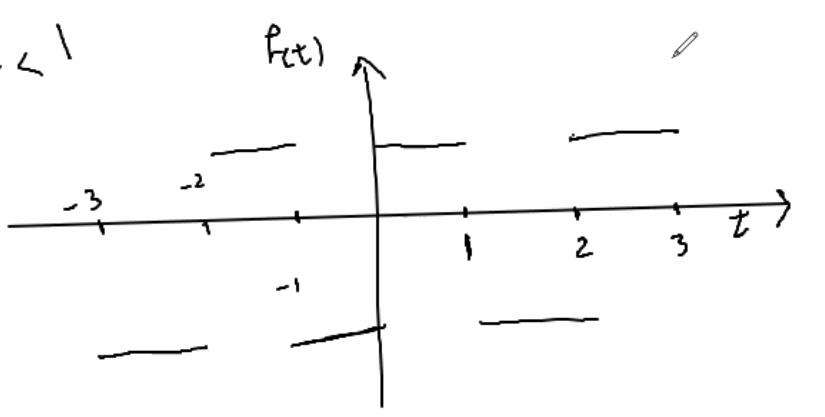
\includegraphics[width = 0.95 \textwidth]{image1.png}

This is a square wave function, and it is odd. 

$f_{odd}(x) \cdot f_{even} (x) = f_{odd} (x)$: An odd function multiplied by an even funciton is an odd function. 

$f_{odd} (x) \cdot f_{odd} (x) = f_{even} (x)$: An odd funciton multiplied by an odd function is an even function. 


If $f(t)$ is an even function:

$$\int_{-L}^L f(t) dt = 2 \int_0^L f(t) dt$$

If $f(t)$ is an odd function:

$$\int_{-L}^L f(t) dt = 0$$

Now, let's find out what the coefficients are of the fourier series. 

$$a_0 = \frac{1}{L} \int_{-L}^L \underbrace{f(t)}_{odd} dt = 0$$

$$a_n = \frac{1}{L} \int_{-L}^L \underbrace{f(t)}_{odd} \underbrace{\cos(\frac{n \pi t}{L})}_{even} dt = 0$$

(note that L = 1)

$$b_n = \int_{-1}^1 f(t) \sin(n \pi t) dt = 2 \int_{0}^{1} (1) \sin(n \pi t) dt = \left. - \frac{2}{n \pi} \cos(n \pi t) \right|_{0}^{1}$$

$$b_n = - \frac{2}{n \pi} \left( \cos(n \pi) - 1 \right) = \frac{4}{(2k - 1) \pi}, \text{with } n = 2k-1 \text{ for } k \in N$$

$$\Rightarrow f(t) = \sum_{k = 1}^\infty \frac{4}{(2k-1) \pi} \sin \left( (2k-1) \pi t \right) = \frac{4}{\pi} \sum_{k = 1}^\infty \frac{\sin \left( (2k-1) \pi t \right)}{2k-1}$$

\subsection{Example 2, part B}

$$f(t) = \begin{matrix} \left\{ \begin{matrix} -t & -2 < t < 0 \\ t & 0 \leq t \leq 2 \end{matrix} \right. & f(t+4) = f(t) \end{matrix} $$

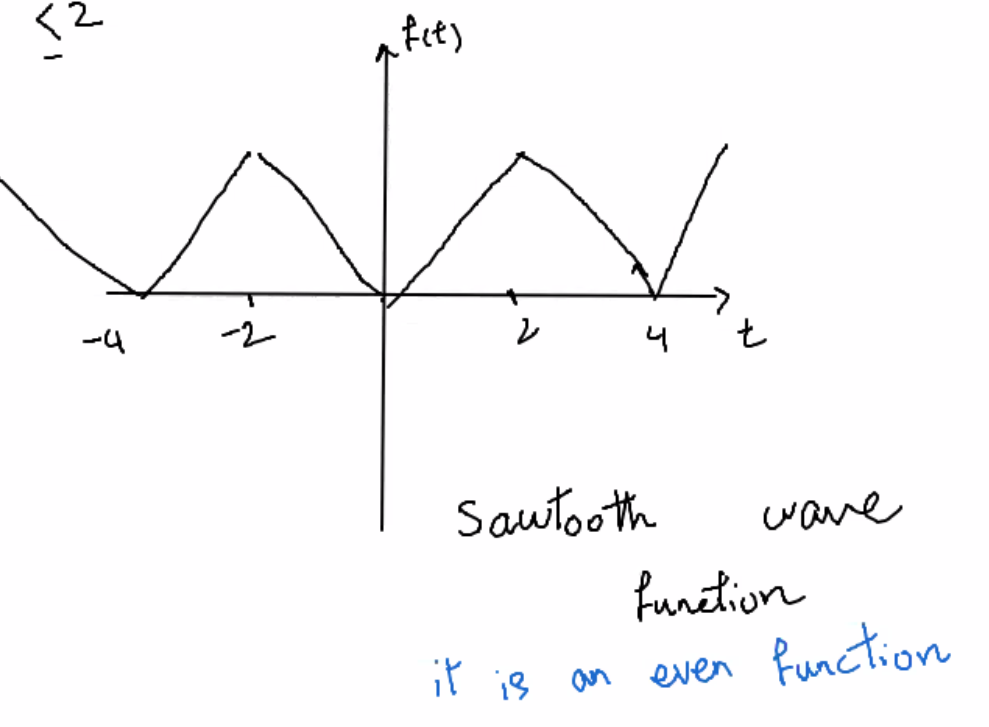
\includegraphics[width = 0.95 \textwidth]{image2.png}

[Note that this is a triangle wave, not a sawtooth wave, but it does not matter for the problem]

$$b_n = 0$$

$$a_0 = \frac{2}{2} \int_{0}^2 t dt = \left. \frac{t^2}{2} \right|_0^2 = 2$$

$$a_n = \frac{2}{L} \int_{0}^2 t \cos (\frac{n \pi t}{2}) dt$$

Using integration by parts, with the following:

$$\begin{matrix} u = t & dv = \cos(\frac{n \pi t}{2}) dt \\ du = dt & v = \frac{2}{n \pi} \sin(\frac{n \pi t}{2}) \end{matrix}$$

$$ = \underbrace{\left. \frac{2}{n \pi} t \sin(\frac{n \pi t}{2} ) \right|_0^2}_{ = 0} - \frac{2}{n \pi} \int_{0}^2 \sin(\frac{n \pi t}{2}) dt = \left. \frac{4}{n^2 \pi^2} \cos(\frac{n \pi t}{2}) \right|_0^2 = \frac{4}{n^2 \pi^2} (\cos(n \pi) - 1)$$

$$\Rightarrow a_n = \frac{-8}{(2k-1)^2 \pi^2}$$

(substituting $n = 2k-1$ above)

$$f(t) = 1 - \frac{8}{\pi^2} \sum_{k = 1}^\infty \frac{\cos \left( \frac{(2k-1) \pi t}{2} \right)}{(2k-1)^2}$$

\textbf{See slides; handwritten before page 6 and pages 6 up to 9 are covered in moderate depth(page numbers based on the numbers at the bottom of the page), and an overview up to the end. Example 3 is an exercise. The last slide is important.}

\section{Fourier Series Slides}

Included here for reference; also available on Canvas under Modules

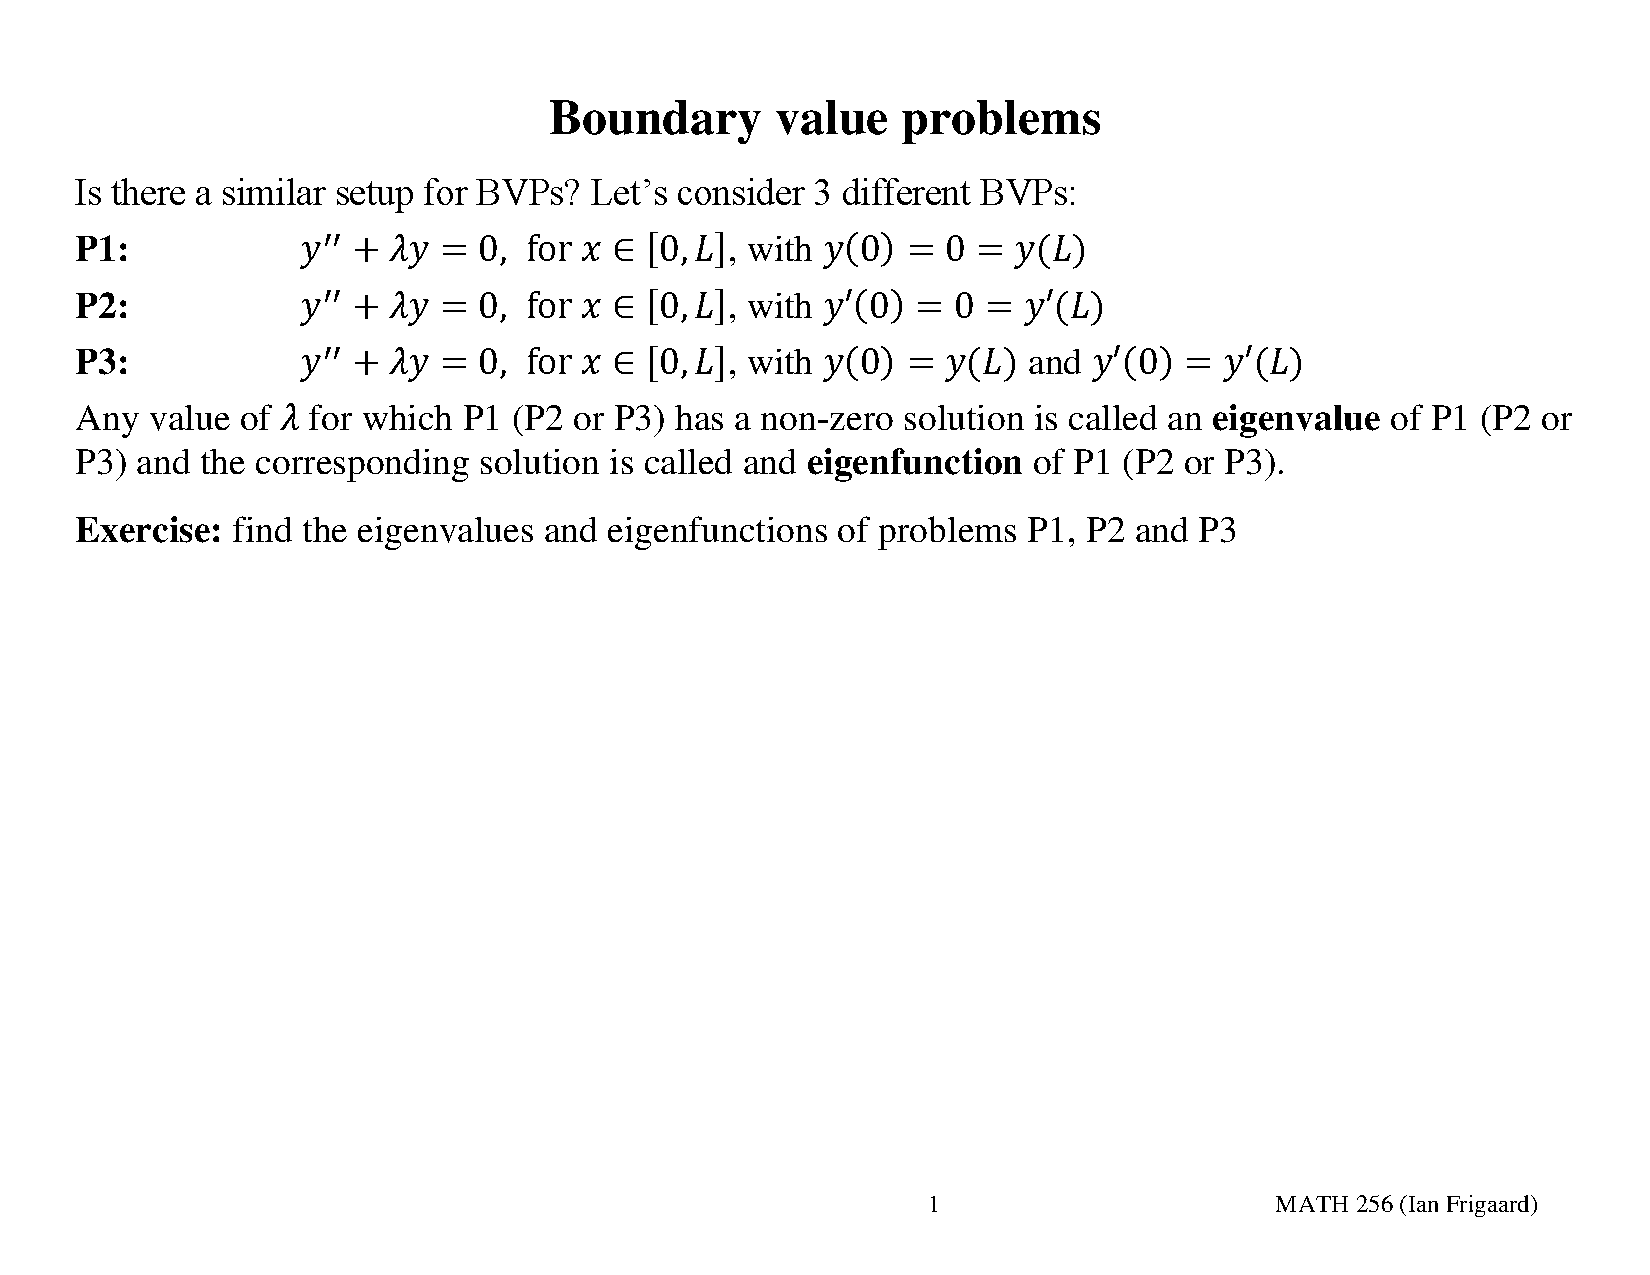
\includepdf[pages=-]{FourierSeries.pdf}


\chapter{Lecture 9}
\graphicspath{{./Lecture9/}}

\section{Recap}

We learned how to write a function as a fourier series, in the following format:

$$f(x) = \frac{a_0}{2} + \sum_{n = 1}^\infty a_n \cos( \frac{n \pi x}{L}) + \sum_{n = 1}^\infty b_n \sin(\frac{n \pi x}{L})$$

We have the following formulas:

$$a_0 = \frac{1}{L} \int_{-L}^L f(x) dx$$

$$a_n = \frac{1}{L} \int_{-L}^L f(x) \cos(\frac{n \pi x}{L}) dx$$

$$b_n = \frac{1}{L} \int_{-L}^L f(x) \sin(\frac{n \pi x}{L}) dx$$

\section{Solving the Heat / Diffusion Equation}

Examples are posted in the pdf slides posted. 

\subsection{Example 1}

Solve the initial boundary value problem (IBVP)
\begin{equation}
\label{Heat Equation}
    \begin{matrix} \frac{\partial u}{\partial t} = \alpha \frac{\partial^2 u}{\partial x^2} & 0 < x < L; & t > 0 \end{matrix}
\end{equation}


$$u(0,t) = u(L,t) = 0$$

$$u(x,0) = f(x)$$

We need to use the method of separation of variables. 

$$u(x,t) = X(x) T(t)$$

Taking the partial derivative with respect to $t$:

$$\rightarrow u_t = X(x) \dot{T} (t)$$

where dots are derivatives with respect to time. 

$$u_x = X'(x) T(t)$$

$$u_{xx} = X''(x) T(t)$$

Now, we substitute this into the PDE equation \ref{Heat Equation}

$$X \dot{T} = \alpha X'' T$$

Now, we divide by $\alpha XT$:

$$\frac{\dot{T}}{\alpha T} = \frac{X''}{X}$$

The left hand side of the equation is a function of $t$, and the right hand side is a function of $x$. In what condition are they equal?

The only way that theycan both be equal is if:
\begin{equation}
\label{Heat constant}
    \frac{1}{\alpha} \frac{\dot{T}}{T} = \frac{X''}{X} = - \lambda
\end{equation}


Where $\lambda$ is a constant. 

\hfill

Now, let's work on boundary conditions:

$$u(0,t) = X(0) T(t) = 0$$

$$u(L,t) = X(L) T(t) = 0$$


\begin{center}
    Hence, $X(0) = X(L) = 0$
\end{center}

From \ref{Heat constant}, we get two equations: 

\begin{itemize}
    \item 1 - BVP
    \item 2 - IVP
\end{itemize}

\subsubsection{BVP}

$$\frac{X''}{X} = -\lambda \Rightarrow X'' + \lambda X = 0$$

with $X(0) = X(L) = 0$. This is a dirichlet boundary condition (BVP type P1)

The solution to P1:

$$X(x) = X_n (x) = C_n \sin(\frac{n \pi x}{L})$$

$$\lambda_n = \left( \frac{n \pi}{L}\right)^2, n \in N$$

Therefore, there is a countably infinite set of $\lambda_n, X_n (x)$ as a solutiojn for the BVP. For each $\lambda_n$ we find an IVP separately:

\subsubsection{IVP}

$$\frac{\dot{T}}{\alpha T} = -\lambda_n \longrightarrow T_n(t) = e^{- \lambda_n \alpha t}$$

is the solution to the IVP. 

\subsubsection{Summary}

We found, for $n = 1,2,3,...$ ($n \in N$), we found:

$$u_n (x,t) = X_n (x) T_n (t) = C_n \sin \left(\frac{n \pi x}{L} \right) e^{- \alpha \left( \frac{n \pi}{L} \right)^2 t}$$

This satisfies $u_t = \alpha u_{xx}$ with the conditions $u(0,t) = u(L,t) = 0$

Since the PDE and boundary conditions are homogeneous, we can superimpose solution, i.e. 

$$C_k u_k + C_m u_m$$


also satisfies this problem for any constants of $C_k$ and $C_m$. 

Let's extend this idea to $\infty$:

$$u(x,t) = \sum_{n = 1}^\infty C_n u_n(x,t) = \sum_{n = 1}^\infty C_n \sin \left( \frac{n \pi x}{L} \right) e^{- \alpha \left( \frac{n \pi}{L} \right)^2 t}$$

for constants $C_1, C_2, C_3,...$. 

\textbf{How abut initial conditions} $u(x,0) = f(x)$?

\begin{equation}
    u(x,0) = \sum_{n = 1}^\infty C_n \sin \left( \frac{n \pi x}{L} \right) = f(x)
\end{equation}

How do we find $C_n$ to meet this condition?

We need to find $C_n$ such that $u(x,0) = \sum_{n = 1}^\infty C_n \sin \left( \frac{n \pi x}{L} \right) = f(x)$ holds. 

If we write $f(x)$ as a fourier sine series, we can match the coefficients. 

Let's write $f(x)$ as a fourier sine series on $[0,L]$: i.e. 


\begin{equation}
    f(x) \approx \sum_{n = 1}^\infty b_n \sin(\frac{n \pi x}{L})
\end{equation}

where $b_n = \frac{2}{L} \int_0^L f(x) \sin \left( \frac{n \pi}{L} x \right) dx$

\hfill

$\Rightarrow$ With comparing (3) and (4) $\rightarrow C_n = b_n$

Finally, the solution for IBVP is:

$$u(x,t) = \sum_{n = 1}^\infty b_n \sin (\frac{n \pi x}{L}) e^{- \alpha \left( \frac{n \pi}{L} \right)^2 t}$$

\begin{itemize}
    \item Homogeneous boundary conditions (Dirichlet: $u(0,t) = u(L,t) = 0$)
    \item Neumann: $u_x(0,t) = U_x (L,t) = 0$
    \item if it's not equal to 0 it's inhomogeneous
    \item If $u_t = \alpha u_{xx} + G$ it's inhomogeneous
\end{itemize}

\subsection{Example 2}

Same as example 1: $f(x) = x(L - x)$, $0 < x \leq L$

To solve, we use the method of separation of variables: $u(x,t) = X(x) T(t)$

Step 1: $u_t = X \dot{T}$; $U_x = X' T$; $U_{xx} = X'' T$

Substitute into PDE and separate variables:

$$X \dot{T} = \alpha X'' T \longrightarrow \frac{\dot{T}}{\alpha T} = \frac{X''}{X} = -\lambda$$

where $\lambda$ is a constant. 

Step 2: Boundary conditions. 

$$\begin{matrix} u(0,t) = 0 \longrightarrow X(0) = 0 \\ u(L,t) = 0 \longrightarrowX(L) = 0 \end{matrix}$$

Step 3: Solve the eigenvalue problem for $X(x)$:

$X'' + \lambda X = 0$, $X(0) = 0 = X(L)$

Hence, the solution:

$$\lambda_n = \left( \frac{n \pi}{L} \right)^2$$

$$X_n = \sin(\frac{n \pi}{L} x)$$

where $n \in N$

Step 4: For each $\lambda_n$ find $T_n(t)$:

$$\frac{1}{\alpha} \frac{\dot{T_n}}{T_n} \rightarrow T_n(t) = e^{- \alpha \lambda_n t} = e^{- \alpha \left( \frac{n \pi}{L} \right)^2 t}$$

Step 5: use superposition and linearity to construct a general series:

$$u(x,t) = \sum_{n  =1}^\infty C_n u_n (x,t) = \underbrace{\sum_{n = 1}^\infty C_n \sin \left( \frac{n \pi x}{L} \right) e^{- \alpha \left( \frac{n \pi}{L} \right)^2 t}}_{X_n(x) T_n(t)}$$

Step 6: Apply initial conditions:

$$u(x,0) = \sum_{n = 1}^\infty C_n \sin (\frac{n \pi x}{L} ) = x(L-x)$$


Write $x(L-x)$ as a Fourier sine series: 

$$x(L-x) = \sum_{n = 1}^\infty b_n \sin (\frac{n \pi x}{L} )$$

$$b_n = \frac{2}{L} \int_0^L x(L-x) \sin \left( \frac{n \pi x}{L} \right) dx$$

$$b_n = \left. - \frac{2}{L} x(L-x) \frac{L}{n \pi} \cos(\frac{n \pi x}{L}) \right|_{0}^{L} + \frac{2}{n \pi} \int_{0}^L (L - 2x) \cos(\frac{n \pi x}{L}) dx$$

$$ = 0 + \frac{2}{n \pi} \int_0^L (L - 2x) \cos \left(\frac{n \pi x}{L} \right) dx = \left. \frac{2L}{(n \pi)^2} (L - 2x) \sin \left(\frac{n \pi x}{L} \right) \right|_{0}^L + \frac{4L}{(n \pi)^2} \int_0^L \sin \left(\frac{n \pi x}{L} \right) dx$$

$$ = \left. \frac{- 4 L^2}{(n \pi)^2} \cos \left(\frac{n \pi x}{L} \right) \right|_0^L = \frac{4L^2}{(n \pi)^3} \left( (-1)^{n+1} + 1 \right)$$

Step 7: Match the initial condition of the series solution ($C_n = b_n$)

$$u(x,t) = \sum_{n = 1}^\infty \frac{4 L^2}{(n \pi)^3} \left( (-1)^{n+1} + 1 \right) \sin \left( \frac{n \pi x}{L} \right) e^{- \alpha \left( \frac{n \pi}{L} \right)^2 t}$$

Note that all $\sin(\frac{n \pi x}{L})$ terms are linearly independent (orthogonal)

\subsection{Example 3}

Similar to example 1 but with Neumann boundary conditions.

\textbf{Please find the examples in the pdf "Heat / diffusion examples" on Canvas}

\begin{center}
    Solution:
\end{center}

Step 1:

$$u(x,t) = X(x) T(t) \rightarrow \frac{\dot T}{\alpha T} = \frac{X''}{X} = -\lambda$$

Step 2:

$$u_x (0,t) = X'(0) T(t) = 0 \rightarrow X'(0) = 0$$

$$u_x (L,t) = X'(L) T(t) = 0 \rightarrow X'(L) = 0$$

Step 3: Solve the BVP with the conditions

$$X'' + \lambda X = 0$$

$$X'(0) = 0 = X'(L)$$

$\Rightarrow$ P2 problem. Cosine series. 

$$\lambda_n = \left(\frac{n \pi}{L} \right)^2$$

and $$X_n(x) = \cos(\frac{n \pi x}{L})$$ for $n \in N$

and $\lambda_0 = 0; X_0 (x) = 1$

\hfill

\hfill

Step 4: Solving the IVP

For each $\lambda_n$ and $X_n$, there is a $T_n$ such that

$$\frac{\dot{T_n}}{T_n} = -\alpha \lambda_n \rightarrow T_n = e^{- \alpha \lambda_n t}$$

Step 5: 

For $\lambda_0 = 0 \rightarrow u_0 (x,t) = 1$

For $\lambda_n = \left(\frac{n \pi}{L} \right)^2 \rightarrow u_n (x,t) = \cos \left(\frac{n \pi x}{L} \right) e^{- \alpha \left(\frac{n \pi}{L} \right)^2 t}$

PDE is linear and homogeneous $\Rightarrow$ we may superimpose the solutions in a linear combination:

$$u(x,t) = \sum_{n = 0}^\infty d_n u_n (x,t) = d_0 + \sum_{n  =1}^\infty d_n \cos \left(\frac{n \pi x}{L} \right) e^{- \alpha \left(\frac{n \pi}{L} \right)^2 t}$$

Step 6: Initial conditions

$$u(x,0) = f(x) = d_0 + \sum_{n =1}^\infty d_n \cos \left(\frac{n \pi x}{L} \right)$$

If we rewrite as a fourier series (cosine), we find that $d_0 = a_0 / 2$ and that $d_n = a_n$

if we take the even extension of $f(x)$, to $[-L, 0]$ interval, then we know $f(x)$ has a fourier cosine series. 

$$f(x) = \frac{a_0}{2} + \sum_{n = 1}^\infty \cos \left(\frac{n \pi x}{L} \right)$$

$$\Rightarrow \begin{matrix} d_0 = \frac{a_0}{2}; & d_n = a_n = \frac{2}{L} \int_0^L f(x) \cos \left(\frac{n \pi x}{L} \right) dx \end{matrix}$$

Step 7:

Thus, the solution is 

$$u(x,t) = \frac{a_0}{2} + \sum_{n = 1}^\infty a_n \cos \left(\frac{n \pi x}{L} \right) e^{- \alpha \left(\frac{n \pi}{L} \right)^2 t}$$

\chapter{Lecture 10}
\graphicspath{{./Lecture10/}}

\section{Recap of Last Lecture}

Last class, we solved homogeneous heat / diffusion PDEs. We used the method of separation of variables, where we assumed $u(x,t)$ can be separated into two functions $X_x$ and $T_t$, such that $u(x,t) = X_x T_t$:

We then substituted that into the PDE, getting two equations; IVP and a BVP. We represented the solutions as a superposition of solutions for each eigenvalue and eigenfunction. 

We then found the coefficients of the Fourier series, or the series of the solution, by writing the initial condition in terms of Fourier series. 

Then we can match up the coefficients and match up the coefficients of the Fourier series into the solution that we found for the PDE. 

Today, we will continue to do more examples. 

\section{Examples}

\subsection{Example 4}

Note that these are the continued examples from the pdf file, named in last class. 1-3 are from last class also. 

$$\begin{matrix} u_t = 0.003 u_{xx} & 0 < x < 1; & t > 0 \end{matrix}$$

$$\begin{matrix} u_x (0,t) = u_x (1,t) = 0 & t > 0 \end{matrix} $$

$$\begin{matrix} u(x,0) = 50x (1-x) & 0 \leq x \leq 1 \end{matrix}$$

How long does it take for $u(0.5,t)$ to obtain its steady-state value, with 1\% error?

\hfill

\hline

\hfill

The solution must be of this form: Note that this is a Neumann boundary condition. 
\begin{equation}
    u(x,t) = d_0 + \sum_{n = 1}^\infty \cos \left(\frac{n \pi x}{L} \right) e^{- \alpha \left( \frac{n \pi }{L} \right) ^2 t}
\end{equation}

Given that $\alpha = 0.003$, $L = 1$, and that $f(x) = 50x (1-x)$, we substitute:

We need to write the Fourier cosine series for $f(x)$:

$$a_0 = \frac{2}{1} \int_0^1 50x(1-x) dx = \left. 100 \left( \frac{x^2}{2} - \frac{x^3}{3} \right) \right|_0^1 = \frac{100}{6}$$

$$a_n = 2 \cdot 50 \int_0^1 x(1-x) \cos \left( \frac{n \pi x}{L} \right) dx = \left. \frac{100}{n \pi} x (1-x) \sin  \left( \frac{n \pi x}{1} \right) \right|_0^1 - \frac{100}{n \pi} \int_0^1 (1-2x) \sin (n \pi x) dx$$

$$a_n = \left. \frac{100}{(n \pi)^2} (1 - 2x) \cos(n \pi x) \right|_0^1 + \frac{200}{(n \pi)^2} \int_0^1 \cos(n \pi x) dx$$

$$a_n = \frac{100}{(n \pi)^2} \left( (-1)^{n+1} - 1 \right)$$

Hence:

$$f(x) = \frac{100}{6} + \sum_{n = 1}^\infty \frac{100}{(n \pi)^2} \left[(-1)^{n+1} - 1 \right] \cos(n \pi x)$$

$d_0 = \frac{50}{6}$ and $d_n = a_n$. This we substitute into (1) and simplify. 


$$u(x,t) = \frac{50}{6} + \frac{100}{\pi^2} \sum_{n = 1}^\infty \frac{\left[ (-1)^{n+1} - 1 \right]}{n^2} \cos(n \pi x) e^{- 0.003 (n \pi)^2 t}$$

As $t \to \infty$, $u(x,t) \to \frac{50}{6}$. This is the steady-state solution. This is also the mean value of the initial condition. (why?)

(n = 2)
\hfill

At $x - 0.5$: $u(x,t) - u(x,\infty) \approx \frac{50}{\pi} e^{-0.0012 \pi^2 t}$, which is $< \frac{1}{100} (\frac{50}{6})$

\hfill

If $0.0012 \pi^2 t > \ln(\frac{600}{\pi^2}) \Rightarrow t > \frac{1}{0.012 \pi^2} \ln \left( \frac{600}{\pi^2} \right) = 34.68 \text{s}$

The plot for the general solution is on the pdf file. 

\section{Inhomogeneous Equations}

In the previous examples, we solved heat / diffusion equations using separation of variables for homogeneous boundary conditions (Neumann and Dirichlet). Now, we are moving on to inhomogeneous equations. 

Either eq: $\frac{\partial u}{\partial t} = \alpha \frac{\partial^2 u}{\partial x^2} + g(x,t)$ or a boundary condition of $u(0,t) = a(t)$ (boundary condition is time dependent), or $u(L,t) = C \neq 0$. 

The idea is to solve these problems by decomposing it into a steady state problem and a homogeneous boundary condition problem, i.e. 

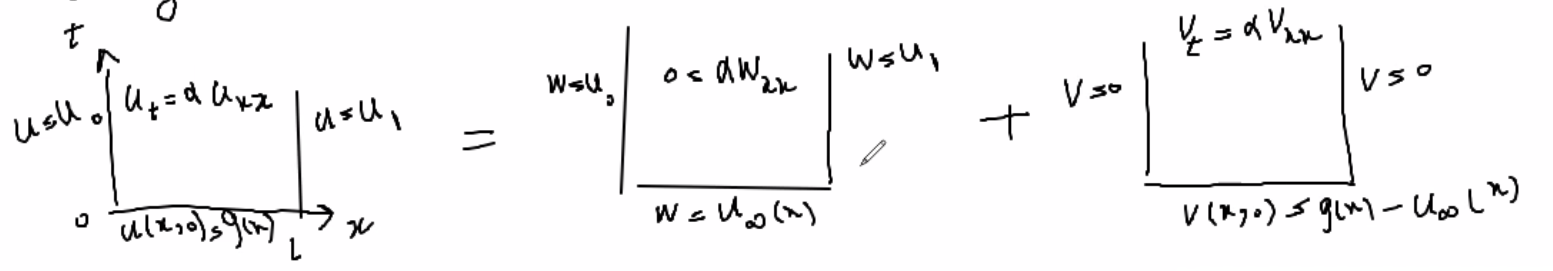
\includegraphics[width = 0.95 \textwidth]{image2.png}

Middle portion is the steady-state problem, and the right hand side is the transient problem with homogeneous boundary conditions. 

The general solution is thus:

$$u(x,t) = w(x) + v(x,t)$$

\subsection{Example 6}

$$\begin{matrix} u_t = \alpha u_{xx} & 0 < t < 1; & t > 0 \end{matrix}$$

$u(0,t) = 1$ and $u(1,t) = 3$ for $t > 0$ and $u(x,0) = x(1-x)$ for $0 \leq x \leq 1$

\subsubsection{Step 1}

We need to decompose the solution into two parts:

$$u(x,t) = \underbrace{u_s (x)}_{\text{Steady-state}} + \underbrace{v(x,t)}_{\text{Transient}}$$

\subsubsection{Step 2}

$$0 = \alpha \frac{\partial^2 u_s}{\partial x^2}$$

$u_s(0) = 1$ and $u_s(1) = 3$ $\rightarrow u_s = A x + B$

$u_s(0) = 1 \rightarrow B = 1$

$u_s(1) = 3 \rightarrow A = 2$

Therefore $u_s = 2 x + 1$

\subsubsection{Step 3}

Formulate $v(x,t)$ and find boundary conditions and initial conditions. 

Boundary conditions:

$v(0,t) = u(0,t) - u_s(0) = 0$

$v(1,t) = u(1,t) - u_s(1) = 0$

Initial conditions:

$$v(x,0) = u(x,0) - u_s(x) = x(1-x) - (2x+1) = -(x^2 + x + 1)$$

$$\frac{\partial u}{\partial t} = \frac{\partial}{\partial t} \left( u_s (x) + v(x,t) \right) = \frac{\partial v}{\partial t}$$

$$\alpha \frac{\partial^2 u}{\partial x^2} = \alpha \frac{\partial^2}{\partial x^2} \left( u_s (x) + v(x,t) \right) = \alpha \frac{\partial^2 v}{\partial x^2}$$

$$\Rightarrow \frac{\partial v}{\partial t} = \alpha \frac{\partial^2 v}{\partial x^2}$$

note: Similar to example 1 and 2, it is a standard (homogeneous) Dirichlet problem. 

\subsubsection{Step 4}

Solve the transient problem. 

$$v(x,t) = \sum_{n = 1}^\infty b_n \sin(n \pi x) e^{-\alpha (n \pi)^2 t}$$

(Refer to example 1 and 2)

$$b_n = \frac{-2}{1} \int_0^1 (1 + x + x^2) \sin(n \pi x) dx = \frac{2}{n \pi} \left[ 3(-1)^n - 1 \right] - \frac{4}{(n \pi)^3} \left[(-1)^n - 1 \right]$$

$$\Rightarrow v(x,t) = \sum_{n = 1}^\infty \left( \frac{2}{n \pi} \left[ 3(-1)^n - 1 \right] - \frac{4}{(n \pi)^3} \left[(-1)^n - 1 \right] \right) \sin(n \pi x) e^{-\alpha (n \pi)^2 t}$$

\subsubsection{Step 5}

Sum the steady state and transient parts of the solution. 

$$u(x,t) = u_x (x) + v(x,t)$$

$$u(x,t) = 1 + 2x + \sum_{n = 1}^\infty \left( \frac{2}{n \pi} \left[ 3(-1)^n - 1 \right] - \frac{4}{(n \pi)^3} \left[(-1)^n - 1 \right] \right) \sin(n \pi x) e^{-\alpha (n \pi)^2 t}$$

\subsection{Example 7}

Inhomogeneous equation and boundary conditions

Equation is given to be the heat equation:

$$\rho c_p \frac{\partial T}{\partial t} = k \frac{\partial^2 T}{\partial x^2} + Q(x)$$

$Q$ is a source (or sink) of heat. 

Let $p = 8940 \frac{kg}{m^3}$, $c_p = 914 \frac{J}{kg \cdot C}$, $k = 930 \frac{W}{m \cdot C}$ $L = 10 m$

Boundary conditions:

$$\begin{matrix} T(10,t) = 30 \\ T(0,t) = 30 \end{matrix}$$

Initial conditons:

$$T(x,0) = 30$$

$$Q(x) = 80000 x$$

Solution:

$$\frac{\partial T}{\partial t} = \alpha \frac{\partial^2 T}{\partial x^2} + q(x)$$

$$\alpha = \frac{k}{\rho c_p} \approx 10^{-4}$$

$$q(x) = \frac{Q(x)}{\rho c_p} = 0.01 x$$

We need to write $u = T(x,t)$

\subsubsection{Step 1}

We need to divide into two parts: 

$$u(x,t) = \underbrace{u_s (x)}_{\text{Steady-state}} + \underbrace{v(x,t)}_{\text{Transient}}$$

\subsubsection{Step 2}

$$0 = \alpha \frac{\partial^2 u_s}{\partial x^2} + q(x)$$

(note that the boundary conditions are $u_s(0) = 30 = u_s(10)$

$$\frac{\partial^2 u_s}{\partial x^2} + 100x = 0 \longrightarrow \frac{\partial u_s}{\partial x} + 50 x^2 = C_1$$

$$u_s = - \frac{50}{3} x^3 + C_1 x + C_2$$

Given boundary conditions: $u_s(0) = 30 \longrightarrow C_2 = 30$ and $u_s(10) = 30 \longrightarrow C_1 = \frac{10^4}{6}$

$$\Rightarrow u_s(x) = - \frac{50}{3} x^3 + \frac{10^4}{6} x = 30$$

\subsection{Step 3}

Formulate the transient part:

Boundary conditions:

$$\left\{ \begin{matrix} v(0,t) = u(0,t) - u_s(0) = 0 \\ v(10,t) = u(10,t) - u_s(10) = 0 \end{matrix} \right.$$

Initial conditions:

$$v(x,0) = 30 - u_s (x) = \frac{10^2}{6} x (x^2 - 100)$$

Double check these!!

Now, we need to solve for $v(x,t)$, which satisfies a standard Dirichlet problem. 

\subsubsection{Step 4}

$$v(x,t) = \sum_{n = 1}^\infty b_n \sin \left( \frac{n \pi}{10} x \right) e^{- 10^{-6} (n \pi)^2 t}$$

$$b_n = \frac{2}{10} \int_0^{10} \frac{10^2}{6} x (x^2 - 100) \sin( \frac{n \pi}{10} x) dx$$

\subsubsection{Step 5}

$$u(x,t) = u_s + v(x,t)$$


\chapter{Lecture 11}
\documentclass{article}

\usepackage{../preamble}
\standalonetrue

\title{MATH 316 Lecture 11}
\author{Ashtan Mistal}
\date{May 31 2021}

\begin{document}

\ifstandalone
\maketitle
\fi

\graphicspath{{./Lecture11/}}

\section{Introduction}

\begin{itemize}
    \item Check Canvas announcements regarding midterm and such (2 new announcements)
\end{itemize}

\section{Recap of Last Lecture}

Last lecture, we finished up the heat / diffusion equation. 

\begin{itemize}
    \item Homogeneous equations and boundary conditions (Neumann and Dirichlet)
    \item Inhomogeneous equations and boundary conditions
    \item Developed general strategies for splitting inhomogeneous equations into a steady state (Which takes care of inhomogeneous parts, incl. boundary conditions) and a transient part (Satisfying a classic homogeneous diffusion equation)
\end{itemize}

\hfill

Today's lecture is about a new equation: Wave equation. 

Two methods to solve:

\begin{itemize}
    \item Applying separation of variables
    \item We'll talk about the second method tomorrow
\end{itemize}

\section{Wave equation}

Takes the following form:

$$y_{tt} = a^2 y_{xx}$$

Two derivatives with respect to time, and two derivatives with respect to $x$. 

Physically, $a = \left[ \frac{T}{\rho} \right]^{\frac{1}{2}}$ (A string under tension), where $T$ is stress / tension, and $\rho$ is density. Can also be written as $a = \left[ \frac{E}{\rho} \right]^{\frac{1}{2}}$ (Elastic bar), where $E = $ elastic stress. 

Boundary conditions: We have two x derivatives $\to$ 2 conditions needed. 

Initial conditions: We also need 2 initial conditions (Because we have 2 time derivatives). This is the main difference between the wave equation and the heat equation.  $y(x,0) = C$ (Initial displacement), and $y_t(x,0) = k$ (initial velocity)

\hfill

Where did the wave equation come from?

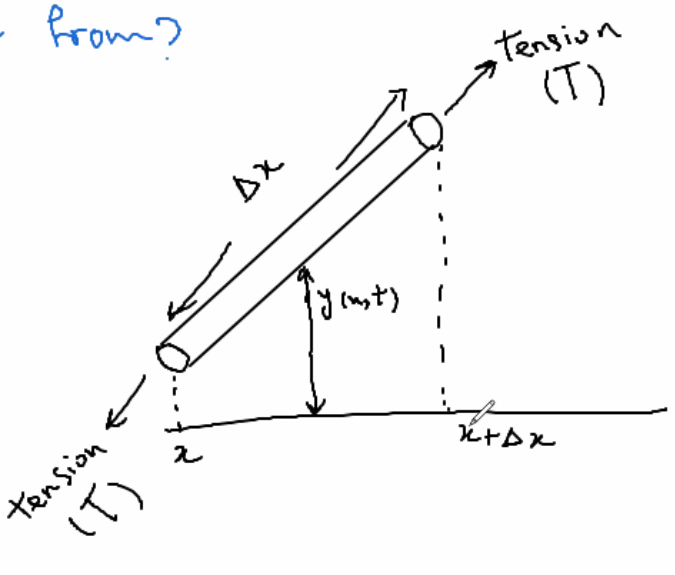
\includegraphics[width = 0.9 \textwidth]{image1.png}

Derivation for small $\left| \frac{\partial y}{\partial x} \right|$

String of density $\rho$ (with units of $\left[ \frac{kh}{m} \right]$)

Force balance in the $y$ direction:

$$\rho \Delta x \frac{\partial^2 y}{\partial t^2} = m \cdot \vec{a} = \sum F_y$$


$$\rho \Delta x \frac{\partial^2 y}{\partial t^2} = T \frac{\partial y}{\partial x} \left( x + \Delta x, t \right) - T \frac{\partial y}{\partial x} (x,t)$$

Divide by $\Delta x$ and let $\Delta x \to 0$:

$$\Rightarrow \rho \frac{\partial^2 y}{\partial t^2} = T \frac{\partial^2 y}{\partial x^2}$$

N.B length of element is $\Delta x (1 + (\frac{\partial y}{\partial x})^2 )^{\frac{1}{2}} \approx \Delta x$

\hfill

\hrule

\hfill

Wave equation: 

$$y_{tt} = a^2 y_{xx}$$

\begin{center}
    BC: $y(0,t) = y(L,t) = 0$
    
    IT: $y(x,0) = f(x)$ and $y_t(x,0) = g(x)$
\end{center}



The idea is to split the solution into two parts. 


\begin{itemize}
    \item Problem 1: Initial velocity, but no displacement of string
    \begin{itemize}
        \item $w_{tt} = a^2 w_{xx}$
        \item $w(0,t) = w(L,t)$
        \item $w(x,0) = 0$ for $0 < x < L$
        \item $w_t(x,0) = g(x)$ for $0 < x < L$
    \end{itemize}
    \item Problem 2: Initial displacement, but no velocity of spring
    \begin{itemize}
        \item $z_{tt} = a^2 z_{xx}$
        \item $z_t (x,0) = f(x)$ for $0 < x < L$
        \item $z_t(x,0) = 0$ for $0 < x < L$
    \end{itemize}
\end{itemize}

Solve problems 1 and 2: $y(x,t) = w(x,t) + z(x,t)$

\subsection{Step 1: Solving Problem 1}

$$w(x,t) = X(x) T(t) \underbrace{\Rightarrow}_{\text{Substitute into PDE}} X \ddot{T} = a^2 X'' T$$

Divide by $a^2 X T$:

$$\Rightarrow \frac{1}{a^2} \frac{\ddot T}{T} = \frac{X''}{X} = - \lambda$$

where $\lambda$ is a constant. 

First, boundary value problem:

$$X'' + \lambda X = 0$$

Boundary conditions are $w(0,t) = X(0) T(t) \Rightarrow X(0) = 0$, and $w(L,t) = X(L) T(t) = 0 \Rightarrow X(L) = 0$

It is a P1 eigenvalue problem. 

Therefore, the eigenvalue problem for $X(x)$ is exactly as for heat / diffusion equation. 

Therefore:

$$\lambda = \lambda_n = \left( \frac{n \pi}{L} \right)^2$$

and $$X_n (x) = \sin \left(\frac{n \pi x}{L} \right)$$

where $n \in \NN$ (Natural numbers; 1,2,3,...)

IVP is:

$$\frac{1}{a^2} \frac{\ddot{T}_n}{T_n} = -\lambda_n \Rightarrow \ddot{T}_n + \left( \frac{a n \pi}{L} \right)^2 T_n = 0$$

Therefore:

$$T_n(t) = A_n \cos \left(\frac{a n \pi}{L} t \right) + B_n \sin \left(\frac{a n \pi}{L} t \right)$$

How about the initial condition?

$w(x,0) = 0 \longrightarrow X(x) T(0) = 0 \Rightarrow T(0) = 0$ and $w_t (x,0) = g(x)$

$T_n (0) = 0 \Rightarrow A_n = 0$

\hfill

As a result:

$$T_n(t) = B_n \sin \left(\frac{a n \pi}{L} t \right)$$

Now, note that PDE, boundary conditions, and $w(x,0)$ are homogeneous. Therefore, we can superimpose solutions. 

$$w(x,t) = \sum_{n = 1}^\infty B_n \sin \left(\frac{n \pi x}{L} \right) \sin \left(\frac{a n \pi}{L} t \right)$$

We need to find $B_n$. To find this, we use the second initial condition. 

$$w_t (x,0) = \sum_{n = 1}^\infty B_n \left(\frac{a n \pi}{L} \right)  \sin \left(\frac{n \pi x}{L} \right) \cos \left(\frac{a n \pi}{L} t \right)$$

$$w_t (x,0) = \sum_{n = 1}^\infty B_n \left(\frac{a n \pi}{L} \right) \sin \left( \frac{n \pi x}{L} \right) = g(x)$$

If we write a Fourier sine series for $g(x)$, we can match up the coefficients:

To make this work, represent $g(x)$ as a Fourier sine series on $\left[ 0, L \right]$:

$$g(x) = \sum_{n = 1}^\infty b_n \sin \left(\frac{ n \pi x}{L} \right) \Rightarrow b_n = \frac{2}{L} \int_0^L g(x) \sin \left( \frac{ n \pi x}{L} \right) dx$$

We know this series converges, so we match up the coefficients. 
\begin{center}
    $B_n = b_n \frac{L}{n \pi a}$ for $n \in \NN$. 
\end{center}


$$\Rightarrow w(x,t) = \sum_{n = 1}^\infty b_n \frac{L}{n \pi a} \sin \left( \frac{n \pi x}{L} \right) \sin \left( \frac{n \pi a t}{L} \right) $$

\subsection{Step 2: Solving Problem 2}

$$z_{tt} = a^2 z_{xx}$$

Initial boundary conditions: $z(0,t) = Z(L,t) = 0$ and $Z(x,0) = f(x)$; $z_t (x,0) = 0$ for $0 < x < L$

Solution: Similarly, we use separation of variables and we assume that $z$ is a product of $X$ and $T$:

$$z(x,t) = X(x) T(t)$$

(Note that these are different X and T than in step 1!!)

The solution for the eigenvalue problem is a P1 problem again. 

$$X_n(x) = \sin \left( \frac{n \pi x}{L} \right)$$
\begin{center}
    $\lambda_n = \left( \frac{n \pi}{L} \right)^2$ for $n \in \NN$
\end{center}


For the IVP part, 

$$\ddot{T}_n + \left( \frac{n \pi a}{L} \right)^2 T_n = 0$$

$$\Rightarrow T_n(t) = A_n \cos \left( \frac{n \pi a}{L} t \right) + B_n \sin \left( \frac{n \pi a}{L} t \right)$$

Now, $z_t(x,0) = X(x) \dot{T}(0) = 0 \Rightarrow \dot{T}_n(0) = 0 \Rightarrow B_n = 0$

So, let's superimpose the solution:

$$z_n (x,t) = \sum_{n = 1}^\infty A_n \sin \left( \frac{n \pi x}{L} \right) \cos \left( \frac{n \pi a}{L} t \right)$$

Use the other initial condition and find $A_n$:

The other initial condition tells us:

$$f(x) = z(x,0) = \sum_{n =1}^\infty  A_n \sin \left( \frac{n \pi x}{L} \right)$$

Suppose we compute the Fourier sine series for $f(x)$, Then, $$b_n' = \frac{2}{L} \int_0^L f(x) \sin \left( \frac{n \pi x}{L} \right) dx$$

\textbf{Note that prime is NOT a derivative, just used to denote that it's a different} $b_n$.

$$\Rightarrow z(x,t) = \sum_{n = 1}^\infty b_n' \sin \left( \frac{n \pi x}{L} \right) \cos \left( \frac{n \pi a}{L} t \right)$$

\subsection{Step 3}

$$y(x,t) = x(x,t) + z(x,t)$$

$$ y(x,t) = \sum_{n = 1}^\infty \left[ b_n \frac{L}{n \pi a} \sin \left( \frac{n \pi x}{L} \right) \sin \left( \frac{n \pi a t}{L} \right) + b_n' \sin \left( \frac{n \pi x}{L} \right) \cos \left( \frac{n \pi a}{L} t \right) \right]$$

We can factor\footnote{Again, $b_n'$ is not a derivative!}:

$$y(x,t) = \sum_{n = 1}^\infty \sin \left( \frac{n \pi x}{L} \right) \left[ \frac{b_n L}{n \pi a} \sin \left( \frac{n \pi a}{L}  t \right) + b_n' \cos \left( \frac{n \pi a}{L}  t \right) \right]$$

\hfill

For Neumann boundary conditions, the procedure is exactly the same as Dirichlet boundary conditions. 

(Using the PDF file posted on Canvas -- Wave Equations, under week 4. Posted at the bottom of this document.)

\section{Example 8}

(Example 8 of the pdf)

Solve the IBVP $y_{tt} = y_{xx}$

Initial conditions: $y(0,t) = y(2,t)$

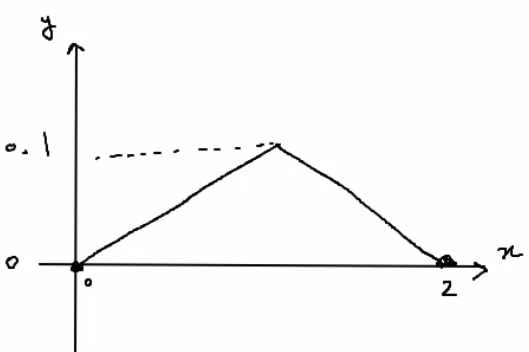
\includegraphics[width = 0.8 \textwidth]{image2.png}

$y(x,0) = \left\{ \begin{matrix} 0.1 x & 0 \leq x \leq 1 \\ 0.1(2-x) & 1 \leq x \leq 1 \end{matrix} \right.$

$y_t (x,0) = 0 = g(x) \Rightarrow b_n = 0$ $ \forall n$

Solution: a = 1 and L = 2. (There is only initialdisplacement $z(x,t)$ problem)

$$b_n' = \frac{2}{L} \int_0^L g(x) \sin \left( \frac{ n \pi x}{L} \right) dx = 0.1 \int_0^1 x \sin \left( \frac{ n \pi x}{2} \right) + 0.1\int_1^2 (2-x) \sin \left( \frac{ n \pi x}{2} \right) $$

$$b_n' = - \frac{0.2}{n \pi} \cos \left( \frac{n \pi}{2} \right) + 0 + \frac{0.4}{(n \pi)^2 } \cdot \left. \sin \left( \frac{n \pi x}{2} \right) \right|_0^1  - 0 + \frac{0.2}{n \pi} \cos( \frac{n \pi}{2}) - \frac{0.4}{(n \pi)^2} \left. \sin  \left( \frac{n \pi x}{2} \right) \right|_1^2$$

$$b_n' = \frac{0.8}{(n \pi)^2 } \sin \left( \frac{n \pi}{2} \right)$$


$$y(x,t) = \sum_{n = 1}^\infty \frac{0.8}{(n \pi)^2 } \sin \left( \frac{n \pi}{2} \right) \sin \left( \frac{n \pi x}{2} \right) \cos \left( \frac{n \pi}{2} t \right)$$

N.B\footnote{Nota bene. Used to denote an important point. }:

$\sin (\frac{n \pi}{2}) = 1,0,-1,0,1,0,...$ for $n \in \NN$

Thus, we could write $n = 2k-1$ and $b_k' = (-1)^{k+1}$ for $k \in \NN$

$$y(x,t) = \sum_{k  =1}^\infty \frac{0.8 (-1)^{k + 1}}{(2k-1)^2 \pi^2} \sin \left( \frac{(2k-1) \pi}{2} x \right) \cos \left( \frac{(2k-1) \pi}{2} t \right)$$

\section{Example 9}

$$y_{tt} = y_{xx}$$

$y(0,t) = 0$ and $y(1,t) = 0$

$y(x,0) = 0$ and $y_t(x,0) = \sin(5 \pi x)$

Solution: a = 1 and L = 1 and $f(x) = 0$ $\Rightarrow$ we only have the velocity problem to solve. 

Need to find the Fourier sine series for $g(x)$:

$$\sum_{n  =1}^\infty b_n \sin(n \pi x) = g(x) = \sin(5 \pi x)$$

But this is already a fourier series. For any $n$ value $\neq 5$, $b_n = 0$. $b_5 = 1$. 

Therefore, the general solution 

$$y(x,t) = \frac{1}{5 \pi} \sin (5 \pi x) \sin(5 \pi t)$$

\section{Wave Equations PDF}


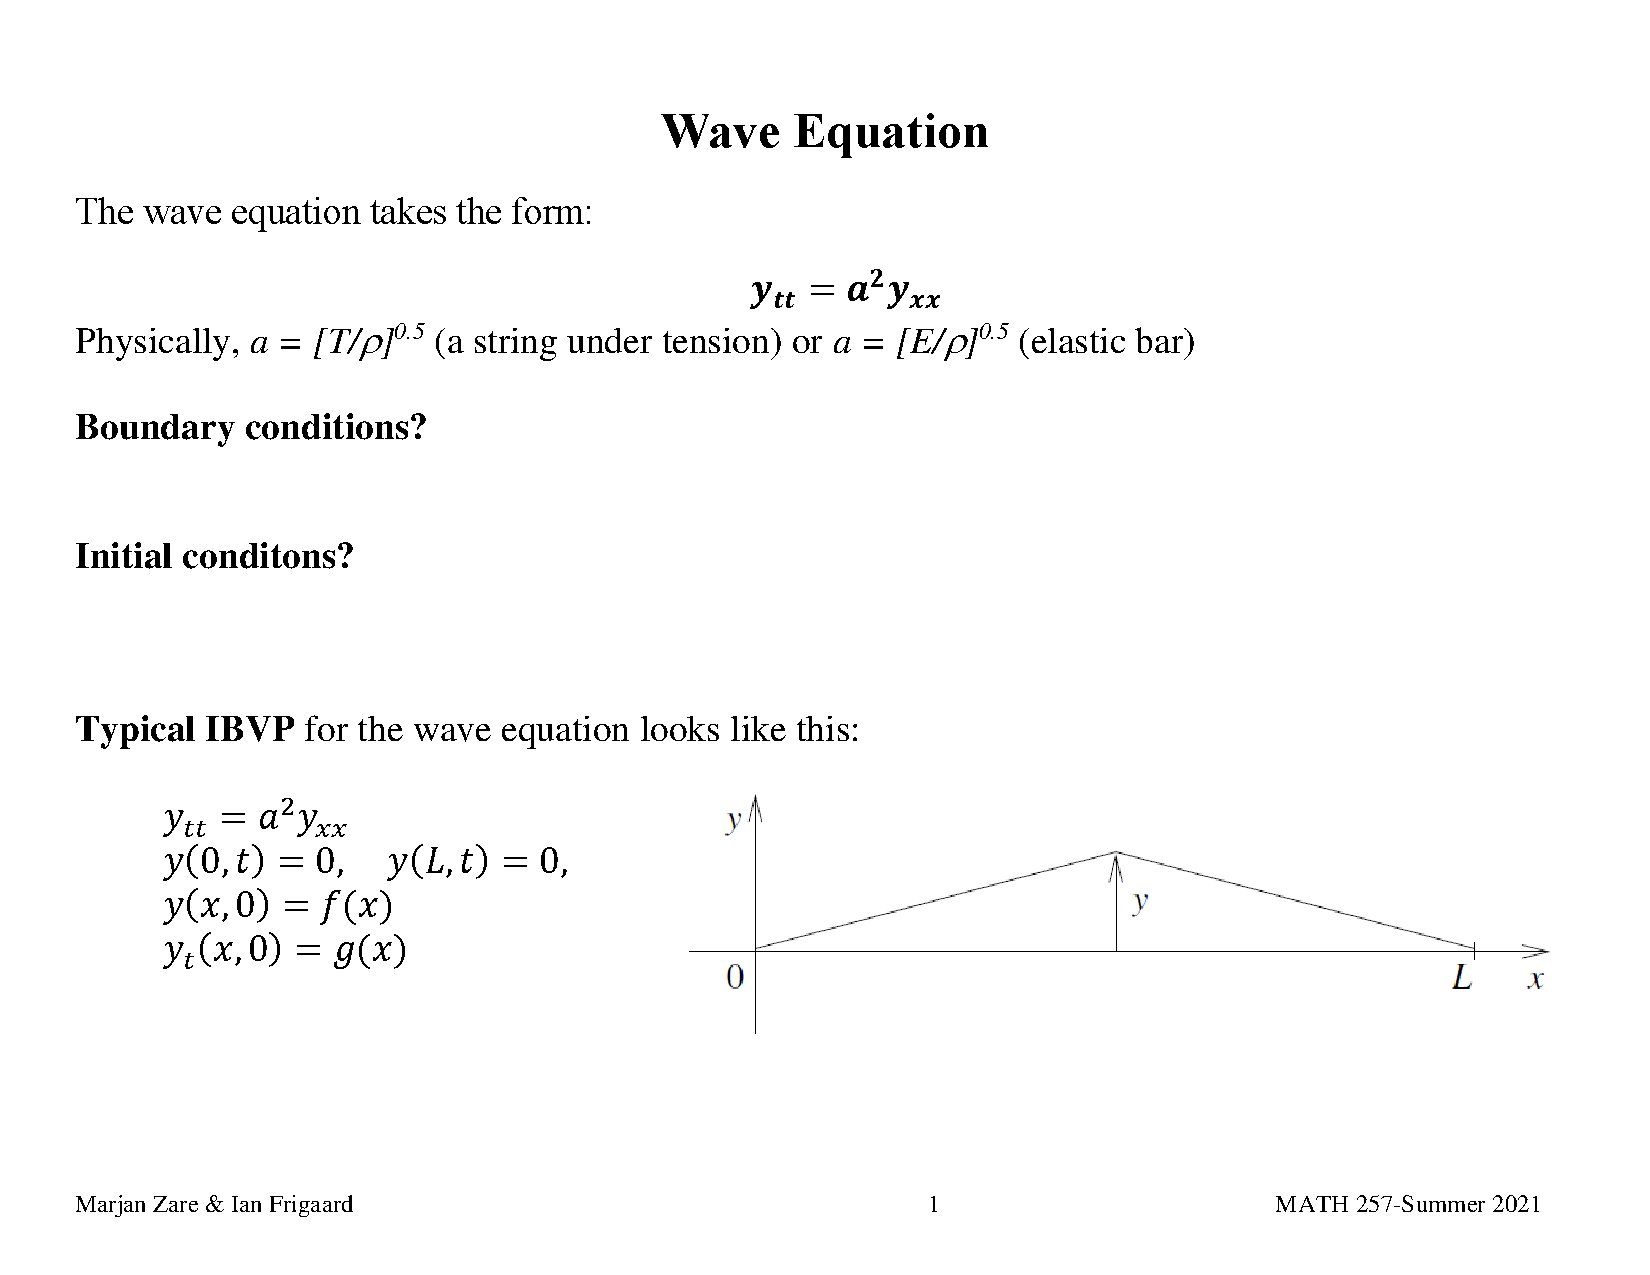
\includepdf[pages=-]{Wave_Equations.pdf}

\end{document}

\chapter{Lecture 12}
\graphicspath{{./Lecture12/}}

\section{Wave Equations: Neumann Boundary Conditions}

Solve IBVP: $y_{tt} = a^2 y_{xx}$

Boundary conditions: $y_x(0,t) = y_x (L,t) = 0$ $\Rightarrow$ Homogeneous Neumann boundary conditions. 

\hfill

Initial conditions: $y(x,0) = f(x)$, $y_t(x,0) = 0 = g(x)$ (Therefore zero initial velocity, with specified initial displacement). 

Split into two problems (w and z). Because $g(x) = 0$, we only have the $z$ equation. For the solution, we use separation of variables. \footnote{Note that left and right side of table are entirely separate. }



$$\begin{array}{l|r}
     X'' + \lambda X = 0 & \ddot T + a^2 \lambda T = 0\\
     \Rightarrow X_n(x) = \cos \left( \frac{n \pi x}{L} \right) & \dot{T}_n (0) = 0 \\
     \lambda_n = \left( \frac{n \pi}{L} \right)^2 & T_n(t) = A_n \cos \left( \frac{n \pi a}{L}  t \right)\\
     X_0(x) = 1 \Rightarrow \lambda_0 = 0 & T_0(t) = 1 
\end{array}$$

The solution would be:

$$y(x,t) = A_0 + \sum_{n = 1}^\infty A_n \cos \left( \frac{n \pi x}{L}  \right) \cos \left( \frac{n \pi a}{L}  t \right)$$

Note that $A_0$ is the multiplication of $X_0 T_0$ terms.

$$\text{At } t = 0 \longrightarrow y(x,0) = A_0 + \sum_{n = 1}^\infty A_n \cos \left( \frac{n \pi x}{L}  \right) = f(x)$$

We construct Fourier cosine series for $f(x)$. 

$$f(x) = \frac{a_0}{2} + \sum{n=  1}^\infty a_n \cos \left( \frac{n \pi x}{L}  \right)$$

$$\Rightarrow A_0 = \frac{a_0}{2}, A_n = a_n$$

\textbf{Note: We can do a similar solution if initial velocity is given. }

\subsection{Recap}

\begin{itemize}
    \item Introduced wave equation
    \item Developed separation of variables method to find its solution
    \begin{itemize}
        \item Dirichlet and Neumann boundary conditions
        \item Examples and normal modes
    \end{itemize}
\end{itemize}

Now: New method. 

\begin{itemize}
    \item New look at the wave equation and we solve the wave equation using \textbf{D'Alembert's solution}. 
\end{itemize}

\section{D'Alembert's Solution}

$$y_{tt} = a^2 y_{xx}$$

Let's see if we can guess a solution of exponential format. 

$$y(x,t) = e^{i k x + \sigma t}$$

where $k$ and $\sigma$ are constants. \footnote{Try this guess solution with heat solution! You will find that it does work for heat equations. }

Substitute the guessed solution into the PDE. 

$$y_tt = \sigma^2 e^{i k x + \sigma t}$$

$$y_{xx} = - k^2 e^{i k x + \sigma t}$$

Now, substitute this into the PDE:

$$\left(\sigma^2 + a^2 k^2 \right) e^{i k t + \sigma t} = 0$$

$$\Rightarrow \sigma = \pm i k a$$

$$y_1 (x,t) = e^{i k (x - at)}$$

$$y_2(x,t) = e^{i k(x + at)}$$

$x \pm at$ are known as characteristics, these are lines in $x$ and $t$ along which the initial conditions (and general information) travels. 

The question here is this: Can this form of solution be more general such that we can apply it to any wave equation?

$$y_1 (x,t) = F(x-at), y_2(x,t) = G(x+at)$$

Can we find a general equation that satisfies the wave equation?


\begin{figure}[ht]
    \centering
    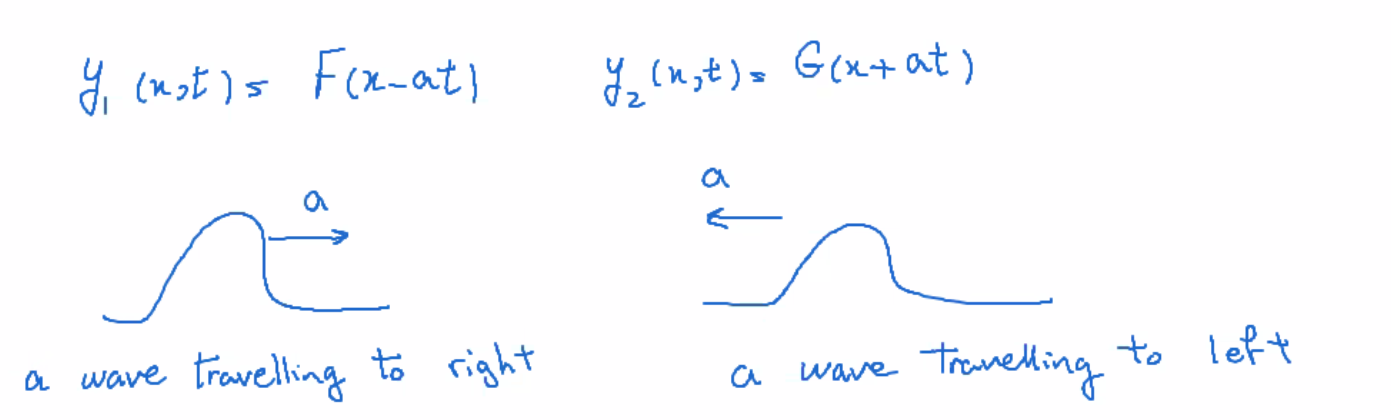
\includegraphics[width = 0.9 \textwidth]{image1.png}
    \caption{$F(x-at)$ is a wave travelling to the right with a speed of $a$. $G(x+at)$ is a wave travelling to the left with a speed of $a$. }
    \label{fig:Wave_directions}
\end{figure}

Hence, a general solution:

$$y(x,t) = F(x-at) + G(x+at)$$

Does it satisfy the PDE?

$$\begin{matrix} y(x,0) = f(x) & \Rightarrow & F(x) + G(x) = f(x) & (1)\\ y_t(x,0) = g(x) & \Rightarrow & -a F'(x) + a G'(x) = g(x) & (2) \end{matrix}$$

We get (2) from:

$$-a F(x) + a G(x) = \int_0^x g(s) ds + A$$

$$(1) xa + 2 \Rightarrow 2aG(x) + f(x) = \int_0^x g(s) ds + A$$

$$\Rightarrow G(x) = \frac{1}{2} f(x) + \frac{1}{2a} \int_0^x g(s) ds + \frac{A}{2a}$$

To find $F(x)$:

$$(1) xa - (2) \Rightarrow 2a F(x) = a f(x) - \int_0^x g(s) ds - A$$

$$\Rightarrow F(x) = \frac{1}{2} f(x) - \frac{1}{2a} \int_0^x g(s) ds - \frac{A}{2a}$$

Now, substitute these into the general solution: (plug into $y(x,t) = F(x-at) + G(x+at)$)

This gives us:

$$\frac{1}{2} f(x-at) - \frac{1}{2a} \int_0^{x-at} g(s) ds + \frac{1}{2} f(x+at) + \frac{1}{2a} \int_0^{x+at} g(s) ds$$

Note that $- \frac{A}{2a}$ and $\frac{A}{2a}$ cancel. 

\begin{equation}
    y(x,t) = \frac{1}{2} \left[ \underbrace{f(x-at)}_{\text{half of init  cond travels right}} + \underbrace{f(x+at)}_{\text{half of init cond travels left}} \right] + \frac{1}{2a} \int_{x-at}^{x+at} g(s) ds
\end{equation}

N.B. Above analysis has no boundary conditions: $-\infty < x < \infty$

\hfill

What if the problem has boundary condition?

Let $F^o (x)$ and $G^o (x)$ be the odd\footnote{ (Assumes Dirichlet boundary conditions)} 2L-periodic extension of $f(x)$ and $g(x)$ respectively:

$$y(x,t) = \frac{1}{2} \left[ F^o (x-at) + F^o (x+at) \right] + \frac{1}{2a} \int_{x-at}^{x+at} G^o (s) ds$$

Boundary conditions: \footnote{Note that we are using the properties of odd functions to cancel out both F and G. }

$$y(0,t) = \underbrace{ \frac{1}{2} \left[ F^o (-at) + F^o (at) \right]}_{=0} + \underbrace{\frac{1}{2a} \int_{-at}^{at} G^o (s) ds}_{ = 0} = 0$$

What's the relationship between D'Alembert's formula and the separation of variables?

$$y(x,t) = \sum_{n = 1}^\infty \sin \left( \frac{n \pi x}{L} \right) \left[ b_n \frac{L}{n \pi a} \sin \left( \frac{n \pi a}{L}  t\right) + b_n' \cos \left( \frac{n \pi a}{L} t \right) \right]$$

Recall trig formulae:

$$\sin(A) \sin(B) = \frac{1}{2} \left[ \cos(A-B) - \cos(A+B) \right]$$

$$\sin(A) \cos(B) = \frac{1}{2} \left[ \sin(A-B) + \sin(A+B) \right]$$

Let's apply these:

$$y(x,t) = \frac{1}{2} \sum_{n  =1}^\infty \frac{b_n L}{n \pi a} \underbrace{\left[ \cos \left( \frac{n \pi}{L} (x-at) \right) - \cos \left( \frac{n \pi}{L} (x+at) \right) \right]}_{\text{Let's write this in integral format}} \rightarrow$$

$$\hookrightarrow + b_n' \left[ \sin \left( \frac{n \pi}{L} (x-at) \right) - \sin \left( \frac{n \pi}{L} (x+at) \right) \right]$$

$$y(x,t) = \frac{1}{2} \sum_{n = 1}^\infty b_n' \left[ \sin \left( \frac{n \pi}{L} (x-at) \right) - \sin \left( \frac{n \pi}{L} (x+at) \right) \right] \rightarrow$$

$$ \hookrightarrow + \frac{1}{2a} \sum_{n = 1}^\infty b_n \int_{x - at}^{x+at} \sin \left( \frac{n \pi s}{L} \right) ds$$

Recall: 

$$\sum_{n = 1}^\infty b_n' \sin(\frac{n \pi x}{L}) = f(x)$$

and

$$\sum_{n  =1}^\infty b_n \sin \left( \frac{n \pi x}{L} \right) = g(x)$$

$\Rightarrow$ d'Alembert's solution:

$$y(x,t) = \frac{1}{2} \left[ f(x-at) + f(x+at) \right] + \frac{1}{2a} \int_{x-at}^{x+at} g(s) ds$$

Both methods give similar solution. 

\end{document}
